
\documentclass[pdftex,a4paper,11pt,DIV15,BCOR20mm,parskip,numbers=noenddot]{scrbook}

\usepackage{default}
\usepackage[ngerman]{babel} % Deutsche Formattierung
\usepackage[T1]{fontenc}
\usepackage[utf8]{inputenc} % Zeichenkodierung
\usepackage[pdftex]{color} % Farben
\usepackage{setspace} % Das Paket setspace ermöglicht ein einfaches Umstellen von normalem, anderthalbfachen oder doppeltem Zeilenabstand.
\usepackage[pdftex]{graphicx} % Bilder
\usepackage[final]{listings}  % ermöglicht die Darstellung von (Programm-)Quellcode in der Arbeit
\usepackage[normalem]{ulem} % ermöglicht das Unterstreichen von Text
\usepackage{amsfonts} % ok-zeichen usw
\usepackage{amsmath} % mathekrams
\usepackage{scrpage2}
\usepackage{babelbib} % Bibliographie
\usepackage{array} % für tabellen
\usepackage[style=base,margin=10pt,font=footnotesize,labelfont=bf]{caption} % Formattierung Bildunterschrift
\usepackage{listings} % Quellcode
\usepackage{float} % floating figures
\usepackage{tikz} % Diagramme
\usepackage{wrapfig} % Text neben Abbildungen
\usepackage{pdflscape} % Seiten in Querformat
\usepackage{geometry}
\usepackage{soul}
\usepackage{textcomp} % Quote Symbol

% schrift auf palatino umstellen
\usepackage{palatino}
\setkomafont{sectioning}{\normalcolor\bfseries} 
% \renewcommand{\familydefault}{\sfdefault}

\definecolor{uhhred}{cmyk}{0,1,1,0}
\definecolor{beige}{RGB}{194,116,31}
\definecolor{green}{RGB}{41,128,38}
\definecolor{brown}{RGB}{132,60,36}
\definecolor{darkblue}{RGB}{38,38,128}

\newcommand{\routput}{\vspace{-0.25cm}\hspace{5pt}\small\color{blue}\ttfamily} 
\newcommand{\rsymbol}{\vspace{-0.25cm}\hspace{5pt}\small\color{blue}\ttfamily\textquotesingle}
\newcommand{\rerror}{\vspace{-0.25cm}\hspace{5pt}\small\color{red}\ttfamily}

\newcommand{\q}{\textquotesingle}
\newcommand{\qq}{\textquotedbl}
    
% Listing-Formattierung
\lstset{
    backgroundcolor=\color{white}, 		% white background
    %     columns=fullflexible, 			% allow latex to break lines
    numbers=none, 				% no line numbering
    showstringspaces=false, 			% no gap character in strings
    belowskip=-10pt, 				% remove blank space at the bottom of listing
    basicstyle=\ttfamily\small\color{darkblue}, 
    xleftmargin=5pt, % Padding
    language=Lisp, 				% for highliting comments and literals
    commentstyle=\color{beige}, 		% comment style
    stringstyle=\color{green}, 			% literal style
    numberstyle=\color{green},
    alsoletter={\#, >},
    keywordstyle=\ttfamily, 			% keyword style
    keywordstyle=[2]\color{green},		% style for literals
    keywordstyle=[3]\color{black},	% style for non-terminals
    literate=
	  *{(}{{{\color{brown}{(}}}}{1} 	% colored brackets
	  {)}{{{\color{brown}{)}}}}{1}	 	
	  {{[}}{{{\color{brown}{{[}}}}}{1}
	  {{]}}{{{\color{brown}{{]}}}}}{1}
	  {\{}{{{\color{brown}{\{}}}}{1}
	  {\}}{{{\color{brown}{\}}}}}{1}
	  {'}{{{\bfseries\color{green}{\textquotesingle}}}}{1}
	  {\#'}{{{\color{green}{\#\bfseries\textquotesingle}}}}{1},
%     % lists of keywords
%     morekeywords={},
    keywords=[2]{\#t, \#f},
    keywords=[3]{\#lang swindle, \#lang racket, >} 
}
  
%   % Tikz styles
%   \usetikzlibrary{shapes,arrows,decorations.markings}
%   \tikzstyle{block} = [rectangle, draw, fill=gray!15, text width=11em, text centered, rounded corners, minimum height=3em]
%   \tikzstyle{label} = [text centered]
%   \tikzstyle{arrow} = [draw, -latex', thick, postaction={decorate}] 
%   \tikzstyle{line} = [draw, -, thick]
  
\usepackage{etoolbox}
\makeatletter
\patchcmd{\chapter}{\if@openright\cleardoublepage\else\clearpage\fi}{}{}{}
\makeatother  
	
\usepackage{colortbl} % für farbige Tabellen
\usepackage{longtable} % für mehrseitige Tabellen
\renewcommand{\arraystretch}{1.25} % in Tabellen: Padding des Textes nach oben und unten in Prozent

% Fußnoten werden im gesamten Dokument fortlaufend hochgezählt und nicht nur kapitelweise, vgl. http://www.golatex.de/nummerierung-der-fussnoten-durchgehend-im-gesamten-dokument-t2042.html
\usepackage{chngcntr}
\counterwithout{footnote}{chapter}

\setlength{\emergencystretch}{1em} % Für den Fall, dass Zeilen im 1. Anlauf nicht richtig umgebrochen werden können, einen 'Notfallraum' einrichten (vgl. http://www.golatex.de/overfull-boxes-in-latex-t1979.html) 

% entnommen aus http://www.siart.de/typografie/latextipps.xhtml#floats
\renewcommand{\floatpagefraction}{0.8} % gibt den Bruchteil einer Seite, die für Gleitobjekte benutzt wird, an, der erreicht werden muss, bevor eine neue Seite angefangen wird. (Standard: 0.5; d.h. wenn ein Bild 51% der Seite einnimmt, wird extra für dieses Bild eine ganze Seite reserviert --> unschön)
\renewcommand{\topfraction}      {0.8}
\renewcommand{\bottomfraction}   {0.5} % \topfraction / \bottomfraction, gibt den Bruchteil einer Seite an, bis zu dem Gleitobjekte oben bzw. unten angeordnet werden sollen.
\renewcommand{\textfraction}     {0.15} % gibt den Bruchteil einer Seite an, der mit Text belegt werden können muss.
\makeatletter
  \setlength{\@fptop}{0pt} % Wenn ein Float-Objekt allein auf einer Seite steht, soll es am oberen Rand der Seite erscheinen und nicht vertikal zentriert
\makeatother

  \usepackage[
%   	pdfstartview={Fit},   
%   	pdffitwindow=true,
  	colorlinks,
  	linkcolor=black,
  	anchorcolor=black,
  	citecolor=black,
  	urlcolor=black,
  	bookmarks, 
  ]{hyperref}
   
% Zeilenabstand
% \setstretch{1.24}   

% Strafpunkte, die beim Seitenumbruch vergeben werden, falls die erste Zeile eines Absatzes allein auf der vorangehenden Seite verbleibt. vgl http://www.jr-x.de/publikationen/latex/tipps/zeilenumbruch.html
\clubpenalty=150

% Strafpunkte, die beim Seitenumbruch vergeben werden, falls die letzte Zeile gerade noch auf die nächste Seite umgebrochen wird. vgl http://www.jr-x.de/publikationen/latex/tipps/zeilenumbruch.html
\widowpenalty=150  

% Pagestyle definieren (nach Martins Template)
\defpagestyle{diplHeadings}
{ % es folgt: Definition des Seitenkopfes: 
  % obere Linie
	(0pt,0pt)
	% linke Seite
	{\upshape \rlap{\pagemark} \hfill \headmark \hfill} % auf einer linken Seite soll LINKS die Seitenzahl stehen und mittig die Headline (headmark)
	% rechte Seite
	{\upshape \hfill \headmark \hfill \llap{\pagemark}} % auf einer rechten Seite soll RECHTS die Seitenzahl stehen und mittig die Headline (headmark)
	% falls Layout "one page"
	{}
	% untere Line
	(\textwidth,1pt)
}
{ % es folgt: Definition des Seitenfußes: Wir wollen lediglich eine schwarze, über die komplette Seite gehende Linie erzeugen
  % obere Linie
	(\textwidth,1pt)
	% linke Seite
	{}
	% rechte Seite
	{}
	% falls Layout "one page"
	{}
	% untere Linie
	(0pt,0pt)
}  
% Pagestyle auch für Chapter-Anfang einrichten
\renewcommand*{\chapterpagestyle}{diplHeadings}
\renewcommand*{\chapterheadstartvskip}{\vspace*{-\topskip}}
\automark[section]{chapter}


% Ränder	
\setlength{\textwidth}{15cm}        % Textbreite
\setlength{\textheight}{24cm}       % Texthöhe
\setlength{\topmargin}{-12mm}       % oberer Rand
\pagestyle{diplHeadings}

\begin{document}

\frontmatter
\newgeometry{centering,left=2cm,right=2cm,top=2cm,bottom=2cm}

\begin{titlepage}
\setcounter{page}{-1}
\includegraphics[scale=0.3]{pictures/logo.pdf}
\vspace*{2cm}
\Large
\begin{center} 
%       {\color{uhhred}\textbf{\so{BACHELORTHESIS}}}
 {\color{uhhred}\textbf{\so{MASTERTHESIS}}}
\vspace*{2.0cm}\\
{\LARGE \textbf{Untersuchungen zur Integration von CLOS-Konzepten in das Objektsystem von Racket}}
\vspace*{2.0cm}\\
vorgelegt von
\vspace*{0.4cm}\\
Manuela Beckert
\end{center}
\vspace*{3.9cm}

\noindent 
MIN-Fakultät \vspace*{0.4cm} \\ 
Fachbereich Informatik \vspace*{0.4cm} \\ 
% Ggf. Professur/Institut \vspace*{0.4cm} \\
Studiengang: Informatik \vspace*{0.4cm} \\ 
Matrikelnummer: 6140959 \vspace*{0.8cm} \\ 
Erstgutachter: Prof. Dr. Leonie Dreschler-Fischer \vspace*{0.4cm} \\ 
Zweitgutachter: Dr. Benjamin Seppke

% Rückseite der Titelseite
\newpage 
\thispagestyle{empty}
\setcounter{page}{0}
~\\ \vfill \noindent 

\end{titlepage}

\restoregeometry


\pagenumbering{Roman}
\setcounter{page}{1}
\pdfbookmark[1]{Inhaltsverzeichnis}{toc}
\tableofcontents
\cleardoublepage 

\pagenumbering{arabic}
\setcounter{page}{1} 
\mainmatter  
\setstretch{1.24}

\chapter{Einleitung} %TODO mehr ausformulieren
An der Universität Hamburg gliedert sich die Lehre zur Softwareentwicklung in zwei Abschnitte. Im ersten Abschnitt werden in den Veranstaltungen ``Softwareentwicklung I'' und ``Softwareentwicklung II'' die Grundlagen für das Programmierverständnis gelegt. Die Studierenden erhalten einen ersten Einblick in imperative und objektorientierte Programmierung in Java nach dem Objects-First-Ansatz.

Anschließend bieten die optionalen Module ``Softwareentwicklung III: Funktionale Programmierung'' sowie ``Softwareentwicklung III: Logikprogrammierung'' zusätzlich die Möglichkeit, zwei weitere  Programmierparadigmen kennenzulernen: funktionale Programmierung am Beispiel von Racket und logikbasierte Programmierung am Beispiel von Prolog.

Racket ist ein Dialekt der funktionalen Sprache Lisp. Genau wie Lisp hat Racket einen funktionalen Kern und ist gleichzeitig eine Mul\-ti\-pur\-pose-Spra\-che. Racket erlaubt es, neben dem funktionalen Stil auch imperative, obkjektorientierte und sogar logikbasierte Programme zu schreiben. Im Rahmen der Lehrveranstaltung werden daher auch diese Möglichkeiten aufgezeigt. 

Racket bietet zwei Arten, objektorientiert zu programmieren: ein integriertes Objektsystem, das sehr ähnlich zu Java ist, und eine Implementation des Common Lisp Object Systems (CLOS), das eine eher funktionalen Sicht auf die Objektorientierung hat. 

Da die Studierenden bereits aus `Softwareentwicklung I'' und ``Softwareentwicklung II'' mit Java vertraut sind, bietet das Objektsystem von Racket bietet kaum neue Lehrinhalte. Aus diesem Grund wird bisher CLOS, das in dem Racket-Dialekt Swindle implementiert ist, behandelt. 

\section{Stand der Forschung} 
\begin{itemize}
 \item ganz knapp: Anfang von OOP (Warum hat man sich das mal überlegt?)
 \item welche Arten von OOP haben sich etabliert? Kernpunkte der Objektsysteme
 \item wichtig: Warum macht man das?
 \item von den Arten zu dem, was man sich ansehen will
 \item vllt. Paper zu CLOS
 \item NICHT Gott und die Welt zitieren! Nur relevantes!
\end{itemize}

\section{Problemstellung} %TODO mehr ausformulieren
Konzepte, die im Modul ``Softwareentwicklung III'' vermittelt werden und die aus dem Objektsystem von Java noch nicht bekannt sind, umfassen: Mehrfachvererbung, Klassenpräzedenzlisten, Methodenkombination und Ergänzungsmethoden.

Es ist bisher nicht möglich, diese Paradigmen aus CLOS in vollem Umfang im Objektsystem von Racket zu verwenden. Beide Systeme verwenden außerdem unterschiedliche Objekte, die nicht ohne weiteres miteinander kommunizieren oder ineinander umgewandelt werden können.

Im Rahmen dieser Arbeit soll eine Racket-Erweiterung entstehen, die Mehrfachvererbung auch im Objektsystem von Racket möglich macht. Der Fokus liegt dabei auf Lehrinhalten des Moduls ``Softwareentwicklung III''.


\section{Vorgehen}
Ein Kapitel zu \textbf{Racket} erläutert, wie die beiden Objektsysteme benutzt werden und beleuchtet die Implementation beider Ansätze. Anschließend wird anhand eines \textbf{Entwurf}s darauf eingegangen, auf welche Weise eine Umsetzung der CLOS-Konzepte im Objekt-System von Racket erfolgen kann und eine entprechende \textbf{Implementation} vorgestellt. Zum Abschluss wird im Kapitel \textbf{Zusammenfassung und Ausblick} über die Umsetzung reflektiert und Möglichkeiten der Erweiterung diskutiert. 
\chapter{Objektsysteme in Racket}
Racket ist ein Dialekt von Lisp, der auf Scheme basiert\cite{racketguide-dialects}. Es ist jedoch keine rein funktionale Sprache, sondern unterstützt verschiedene Lisp-Dialekte und  Programmierparadigmen. 
%Damit gibt Racket Programmierern und Forschern die Werkzeuge, die sie benötigen, um neue Sprachen zu erkunden und zu entwickeln\cite{racketguide-dialects} und wird beispielsweise auch an der Universität Hamburg in der Forschung genutzt.

Racket wird in der Softwareentwicklungslehre genutzt, da es im Gegensatz zu Common Lisp sehr einsteigerfreundlich ist. Die Veranstaltungsteilnehmer lernen zum ersten Mal eine funktionale Sprache kennen und sollen einen möglichst einfachen Einstieg erhalten. Hierzu bietet Racket eine übersichtliche Syntax und eine plattformunabhängige Entwicklungsumgebung, die vergleichbare Fehlermeldungen liefert.

In Common Lisp wird die Syntax schnell sehr komplex und ist zudem abhängig von der Implementierung (teilweise sogar mit kostenpflichtigem Interpreter). Common Lisp hat zwei verschiedene Paketsysteme mit tausenden von Paketen, was ein schnelles Zurechtfinden in der Sprache nicht unbedingt begünstigt. Es gibt keine dedizierte grafische Oberfläche, da Common Lisp für die Integration in Emacs, Vim etc. ausgelegt ist. Das würde bedeuten, dass Veranstaltungsteilnehmer sich erst einmal mit der Integration der Sprache in den Editor ihrer Wahl beschäftigen müssten, bevor sie überhaupt eine Zeile Code schreiben können. Nicht alle Interpreter von Common Lisp werden auch für alle Betriebssysteme gewartet, wie zum Beispiel SBCL, der zwar frei und gut ist, aber unter Windows nur gelegentlich gepflegt wird. Das macht es extrem schwer die Ursache von Fehlern zu erkennen, da immer auch das Betriebssystem bedacht werden muss. Zudem ist eine systemübergreifende grafische Ausgabe ohne weitere Pakete nicht vorgesehen. Das erschwert das Stellen von Aufgaben, bei denen das Ergebnis visualisiert werden kann oder muss, da die grafische Ausgabe vom Interpreter abhängig ist und die Teilnehmer zudem erst einmal die entprechenden Pakete installieren müssten. 

Um Common Lisp zu lernen, wurde daher Scheme entwickelt. Analog zu BlueJ, einer Entwicklungsumgebung für das Lernen von objektorientierter Programmierung in Java, war DrScheme das Einsteigertool zu Common Lisp. Im Jahr 2010 wurde Scheme umbenannt zu Racket. Racket bildet einen guten Kompromiss für die Lehre, da es einen einfachen Einstieg in die Welt von Common Lisp bietet.
%----------------------

Die Syntax von Racket ist sehr ähnlich zu Common Lisp. Ausdrücke werden geklammert, Kommentare mit einem Semikolon eingeleitet. Einige Standardfunktionen haben leicht abgewandelte Namen. So werden in Racket beispielsweise sowohl Funktionen als auch Variablen mit dem Schlüsselwort \texttt{define} definiert, anstelle von \texttt{defun}, \texttt{defvar} und \texttt{defparameter} in Common Lisp. Prädikate enden auf \texttt{?} (zum Beispiel \texttt{equal?}) und Methoden, die Variablen oder Objekte verändern auf \texttt{!} (zum Beispiel \texttt{set!}). Einer der größeren Unterschiede liegt in der Art, wie Makros definiert werden; darauf wird im Kapitel \ref{makros} noch näher eingegangen.

Racket unterstützt auch objektorientierte Programmierung auf zwei verschiedene Arten. Zunächst gibt das Racket-Objektsystem. Racket-Klassen sind sehr ähnlich zu Klassen in Java, C\# oder den meisten objektorientierten Programmiersprachen\cite{neu-edu2}. Ein Programm kann Klassen definieren, instanziieren, mit den erzeugten Objekten interagieren und Klassen erweitern. Besonders ist, dass Klassen auch wie Funktionswerte behandelt werden können. Es ist möglich, eine Klasse zur Laufzeit zu erweitern, eine Klasse an eine Funktion zu geben oder in einer Datenstruktur zu speichern und anschließend abzufragen\cite{neu-edu}. 

Zusätzlich gibt es den Racket-Dialekt Swindle, in dem das Common Lisp Object System (CLOS) implementiert ist. Im Gegensatz zum eingebauten Objektsystem von Racket bietet CLOS Funktionalitäten wie Mehrfachvererbung, Methodenkombination oder Ergänzungsmethoden. Durch die Implementation als Metaobject-Protocol bietet es dem Programmierer zudem viel Freiheit bei der Erweiterung und Veränderung der Repräsentation von Klassen und Objekten.
Um ein Gefühl für die beiden Objektsysteme zu bekommen, soll zunächst betrachtet werden, wie sie benutzt werden können. %Andschließend wird ein Blick auf die Implementation beider Ansätze geworfen. Die Autoren des Buches ``The Art of the Metaobject Protocol''\cite{amop} vergleichen das Vorgehen sehr treffend mit eine Theateraufführung: Auf der Bühne (onstage) findet das Theaterstück statt - das Programm, oder etwas allgemeiner, das, was der Programmierer von der Sprache sieht. Hinter der Bühne (backstage) befindet sich die darunterliegende Implementation, die die entprechenden Makros definiert und mit für den Programmierer nicht sichtbaren Objekten und Funktionen arbeitet. Wir wollen beide Ansätze erst ``onstage'' betrachten bevor wir einen Blick hinter die Kulissen werfen.

Der Fokus dieser Arbeit liegt auf der Implementation von Mehrfachvererbung im Objektsystem von Racket. Natürlich bieten sowohl das Objektsystem von Racket als auch CLOS neben Vererbung auch noch viele weitere nützliche Funktionen und Eigenschaften; diese sind jedoch nicht zielführend für diese Arbeit und es würde eine eigene Ausarbeitung benötigen, sie alle aufzulisten. Im Folgenden wird daher nur auf diejenigen Bestandteile beider Ansätze eingegangen, die direkt oder indirekt mit Mehrfachvererbung zu tun haben. 

Die Installation von Racket beinhaltet eine integrierte Enwicklungsumgebung namens DrRacket. Für das Syntaxhighlighting der Quelltextbeispiele in dieser Arbeit wurde das Standard-Farbschema von DrRacket verwendet. Anfragen an die Interaktionskonsole wurden mit \texttt{>} markiert und das Ergebnis in der Zeile darunter aufgeführt. 

\section{Beispielproblem} 

%TODO Beispielproblem überarbeiten 

Beide Objektsysteme sollen anhand eines Beispielproblems beschrieben werden. Es soll zunächst das Verhalten einfacher Klassen und Einfachvererbung gezeigt werden und darauf aufbauend die Konzepte von Mehrfachvererbung, die in den Objektsystemen vorhanden sind. Ziel wird es daher sein, die folgende Vererbungshierarchie zu implementieren:

\begin{figure}[h]
 \centering
 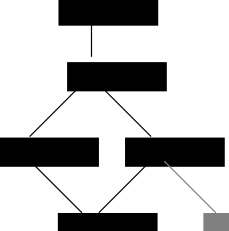
\includegraphics[width=0.35\textwidth]{pictures/hirarchy}
 \caption{Vererbungshierarchie für die Klasse Pokemon.}
 \label{hirarchy}
\end{figure}

Die Klasse Thing soll eine einfache Basisklasse sein und uns die Möglichkeit geben, die Syntax der Klassendefinition beider Ansätze zu vergleichen. Da Thing ledigleich eine leere Klasse ist, wollen wir im Anschluss zwei Klassen erstellen, deren Felder und Methoden später vererbt werden können: Element und Animal. Anhand von Element betrachten wir dabei zunächst, wie Felder und Methoden definiert werden können. Anhand der Klasse Animal und ihrer Subklasse Pet können wir das Konzept der Vererbung veranschaulichen. Es wird dann mit der Klasse Pokemon gezeigt, welche Möglichkeiten der Mehrfachvererbung es gibt.

Zusätzlich soll für beide Objektsysteme geprüft werden, welche Möglichkeiten es gibt, Methoden einer Superklasse in einer Subklasse zu ergänzen. 
\section{Das Objektsystem von Racket}
Als Grundlage für dieses Kapitel dient die Racket-Dokumentation \cite{racketguide-classes} und -Referenz \cite{racketref-classes} für Klassen und Objekte.

Racket ist eine Multipurpose-Sprache und erlaubt die Auswahl der Syntax auf Sprachebene. Eine einzelne Codezeile bestimmt die Sprache eines Moduls, also beispielsweise, ob die Funktionen vorgezogen ausgewertet werden (\texttt{\#lang racket}) oder verzögert (\texttt{\#lang lazy}). Da das Objektsystem in die Sprache Racket integiert ist, kann man es direkt in jedem Racket-Modul verwenden.

Die wichtigsten Werkzeuge, die man als Programmierer in einer objektorientierten Sprache benötigt, sind das Definieren von Klassen, Feldern und Funktionen, sowie das Erzeugen von Objekten. Auf diese soll deshalb im Folgenden kurz eingegangen werden, bevor wir dazu kommen, welche Möglichkeiten es in Bezug auf Mehrfachvererbung im Objektsystem von Racket bereits gibt.

Alle Code-Beispiele befinden sich auch auf der beiligenden CD und sind noch einmal zusammenhängend in Anhang \ref{or-example} aufgeführt. 

\subsection{Einfache Klassen}

Eine Klasse wird in Racket durch das Schlüsselwort \texttt{class} definiert. Bei der Definition einer Klasse muss die Superklasse angegeben werden. Falls die Klasse keine (andere) Superklasse hat, wird \texttt{object\%} angegeben, die eingebaute Wurzelklasse. Per Konvention sollen Klassennamen in Racket auf \% enden, bei den folgenden Beispielen wird jedoch darauf verzichtet, um sie später leichter mit CLOS vergleichen zu können. Nach der Superklasse können noch beliebige Klassenoptionen, Felder oder Methoden definiert werden. An einer beliebigen Stelle im Rumpf der Klasse muss jedoch mit \texttt{super-new} der Konstruktor der Oberklasse aufgerufen werden. Eine minimale Klassendefinition sieht damit folgendermaßen aus:

\begin{lstlisting}
(class object% (super-new))
\end{lstlisting}

Als Rückgabewert erhält man ein Klassenobjekt und kann dieses für den späteren Zugriff einer Variablen zuweisen. Wir können die leere Klasse beispielsweise Thing nennen.

\begin{lstlisting}
(define Thing (class object% (super-new)))
\end{lstlisting}

Objekte von Klassen lassen sich mit den Schlüsselwörtern \texttt{new}, \texttt{make-object} und \texttt{instantiate} erzeugen, je nachdem ob Initialisierungsargumente durch Name, Position oder auf beide Arten angegeben werden sollen. Wir verwenden im Folgenden \texttt{new} und initialisieren damit Felder durch Angabe des Namens:

\begin{lstlisting}
(new Thing)
\end{lstlisting}

Felder lassen sich mit \texttt{init-field} oder \texttt{field} deklarieren, je nachdem, ob es möglich sein soll sie bei der Objekterzeugung zu initialisieren oder nicht. Wir können beispielsweise zu der Klasse Thing ein Feld hinzufügen, das eine Beschreibung des Objekts enthält:

\begin{lstlisting}
(define Thing (class object% (super-new)
                (init-field [name "a Thing"])))
\end{lstlisting}

Auf die Felder kann man dann mit \texttt{get-field} beziehungsweise \texttt{set-field!} zugreifen. 

\begin{lstlisting}
> (get-field name (new Thing))
\end{lstlisting}
{\routput {\qq}a Thing{\qq}}

\begin{lstlisting}
(define bob (new Thing [name "Bob"]))

> (get-field name bob)
\end{lstlisting}
{\routput {\qq}Bob{\qq}}

\begin{lstlisting}
> (set-field name bob "not Bob")
> (get-field name bob)
\end{lstlisting}
{\routput {\qq}not Bob{\qq}}

Für Methoden gibt es, je nach Art und Sichtbarkeit, unter anderem die Schlüsselwörter \texttt{define/public}, \texttt{define/private} und \texttt{define/override}. Wir können für die Klasse Thing eine Methode \texttt{who-are-you?} definieren, die einen beschreibenden Text für das Objekt ausgibt:

\begin{lstlisting}
(define Thing (class object% (super-new)
                (init-field [name "a Thing"])
                (define/public (who-are-you?) 
                  (string-append "I am " name "!"))))
\end{lstlisting}

Die Methode lässt sich anschließend mittels \texttt{send} aufrufen.

\begin{lstlisting}
(send (new Thing) who-are-you?)
\end{lstlisting}
{\routput {\qq}I am a Thing!{\qq}}

\begin{lstlisting}
(send bob who-are-you?)
\end{lstlisting}
{\routput {\qq}I am not Bob!{\qq}}

Attribute, die keinen Defaultwert haben, müssen bei der Initialisierung angegeben werden. Da das Attribut \texttt{name} den Wert  \texttt{{\qq}a Thing{\qq}} als Defaultwert hat, ist eine Angabe bei der Objekterzeugung optional. 

Um von Thing zu erben, müssen wir in der Klassendefinition lediglich Thing statt \texttt{object\%} als Superklasse angeben. So können wir beispielweise eine Klasse Element definieren, die von Thing erbt:

\begin{lstlisting}
(define Element (class Thing (super-new)
                  (init-field [attr 'water])
                  (define/public (hot?) (equal? attr 'fire))))
\end{lstlisting}

Element definiert auch noch ein eigenes Feld sowie eine Methode, damit wir später das Verhalten bei der Klasse betrachten können, die von Element erbt. Objekte von Element haben sowohl Zugriff auf die neu definierten Features als auch auf die geerbten:

\begin{lstlisting}
> (send (new Element) who-are-you?)
\end{lstlisting}
{\routput {\qq}I am a Thing!\qq}

\begin{lstlisting}
(define elem (new Element "Fire" 'fire))
> (send elem who-are-you?)
\end{lstlisting} 
{\routput {\qq}I am Fire!\qq}
\begin{lstlisting}
> (send elem hot?)
\end{lstlisting} 
{\routput{\#t}}

Element kann auch das geerbe Verhalten von Thing ändern. Wenn wir zum Beispiel den Defaultwert von \texttt{name} in Element ändern wollen, können wir den Wert per Hand mit \texttt{init} initialisieren und den Wert dann an die Superklasse übergeben:

\begin{lstlisting}
(define Element (class Thing 
                  (init [name "an Element"])  ; !
                  (super-new [name name])     ; !
                  (init-field [attr 'water])
                  (define/public (hot?) (equal? attr 'fire))))
  
(send (new Element) who-are-you?)
\end{lstlisting}
{\routput {\qq}I am an Element!\qq}

Analog können geerbte Methoden mit \texttt{define/override} überschrieben werden. Die Methode der Superklasse lässt sich mit \texttt{super} aufrufen:

\begin{lstlisting}
(define Element (class Thing 
                  ...
                  (define/override (who-are-you?)
                    (string-append (super who-are-you?)
                                   (if (hot?) " And I am hot!" "")))))
                                   
> (send (new Element) who-are-you?)
\end{lstlisting}
{\routput {\qq}I am an Element!\qq}

\begin{lstlisting}
> (send elem who-are-you?)
\end{lstlisting}
{\routput {\qq}I am Fire! And I am hot!\qq}

Es gibt jedoch eine Einschränkung: Features der Oberklasse sind innerhalb der Klassendefinition von Element jedoch nicht ohne weiteres sichtbar: 

\begin{lstlisting}
(define Element (class Thing 
                  ...
                  (define/public (get-name) name)))
\end{lstlisting}
{\rerror class: cannot use non-field init variable in a method in: name}

Wir haben Felder und Methoden der Superklasse bisher immer innerhalb eines \texttt{super}-Aufrufs benutzt. Falls wir jedoch direkten Zugriff auf den Wert von \texttt{name} brauchen, so müssen wir das explizit durch \texttt{inherit-field} (oder \texttt{inherit} für Methoden) angeben:

\begin{lstlisting}
(define Element (class Thing 
                  (init [name "an Element"])
                  (super-new [name name])
                  ...
                  (inherit-field name)
                  (define/public (get-name) name)))
\end{lstlisting}
{\rerror  class: duplicate declared identifier in: name}

Wir erhalten immer noch einen Fehler, denn nun haben wir zwei Deklarationen für das Feld \texttt{name}: durch \texttt{init} und durch \texttt{inherit-field}. Wir müssen uns entscheiden, eins von beiden umzubennennen. Ein Umbenennen des Initialisierungs-Paramters würde bedeuten, dass sich die Syntax der Objekterzeugung ändert, das wollen wir vermeiden. Es wird also das geerbte Feld umbenannt:

\begin{lstlisting}
(define Element (class Thing 
                  ...
                  (inherit-field [newname name])
                  (define/public (get-name) newname)))
\end{lstlisting}

Nun gibt es keinen Fehler mehr und wir können die Methode aufrufen:

\begin{lstlisting}
> (send (new Element) get-name)
\end{lstlisting}
{\routput {\qq}an Element\qq}

\subsection{Mehrfachvererbung in Racket}
\label{mixins}
Zuvor wurde behauptet, mit Racket könne man keine Mehrfachvererbung modellieren. Tatsächlich gibt es zwei Arten von Klassen in Racket, deren Verhalten auf den ersten Blick wie Mehrfachvererbung aussieht: Mixins und Traits. Es werden deshalb beide kurz vorgestellt, um aufzuzeigen, welche Probleme und Grenzen sie haben.

Dafür verwenden wir unsere vorher definierte Klasse Thing, eine vereinfachte Version von Element, sowie die folgende Klasse Animal, die ebenfalls von Thing erbt:

\begin{lstlisting}
(define Element (class Thing 
                  (init [name "an Element"])
                  (super-new [name name])
                  (init-field [attr 'water])
                  (define/public (hot?) (equal? attr 'fire)))

(define Animal (class Thing
                 (init [name "an Animal"])
                 (super-new [name name])
                 (init-field [size 'small])))
\end{lstlisting}

Animal redefiniert ebenfalls den Defaultwert für den Namen und besitzt außerdem noch ein eigenes Feld \texttt{size} für die Größe.

Animal und Element haben sowohl gemeinsame als auch unterschiedliche Felder und Methoden. Wir wollen versuchen, die Felder und Methoden aus beiden in einer neuen Klasse namens Pokemon zu vereinigen. 

% Das ginge natürlich ganz simpel, indem eine der beiden Klassen in Pokemon umbenannt wird und von der anderen erbt, deshalb wollen wir außerdem fordern, dass beide Klassen auch einzeln verwendet können. 


\subsubsection{Mixins}
Die Auswertung eines \texttt{class}-Aufrufs gibt uns ein Klassenobjekt zurück. Es möglich, dieses als Parameter an Funktionen oder andere Klassen zu übergeben oder auch als Rückgabewert eines Funktionsaufrufs zu definieren. Wir könnten uns beispielsweise eine Methode \texttt{generate-subclass} definieren, die eine Klasse als Parameter erhält und eine Subklasse von dieser erzeugt. Dafür muss sie den Parameter nur als Superklasse in einer Klassendefinition verwenden:

\begin{lstlisting}
(define (generate-subclass superclass)
  (class superclass (super-new)))
\end{lstlisting} 

Das ist noch keine sonderlich spannende Subklasse, da sie sich genauso verhält wie die angegebene Superklasse.
% aber wir können uns von ihrer Funktionalität überzeugen. Nehmen wir beispielsweise eine Subklasse der Klasse Element:
% 
% \begin{lstlisting}
% > (generate-subclass Element) 
% \end{lstlisting}
% {\routput \#<class:...>}
% 
% Dann erhalten wir das gleiche Verhalten wie für Objekte der Klasse Element:
% 
% \begin{lstlisting}
% > (new (generate-subclass Element))
% \end{lstlisting}
% {\routput (object:...)}
% 
% \begin{lstlisting}
% > (send (new (generate-subclass Element)) get-attr)
% \end{lstlisting}
% {\rsymbol water}
% 
Nun könnte man in der in \texttt{generate-} \texttt{subclass} definierten Klasse natürlich auch noch weitere Felder und Methoden hinzufügen. Die Klasse fügt dann Verhalten zu einer bestehenden, aber noch unbekannten Klasse hinzu. Erst beim Methodenaufruf wird der Platzhalter mit einer tatsächlichen Superklasse gefüllt. Eine solche Klasse wird in Racket Mixin genannt und als Platzhalter für die Superklasse wird per Konvention \texttt{\%} genommen:

\begin{lstlisting}
(define (a-mixin %)
  (class % (super-new)
    ; neues Verhalten
    ))
\end{lstlisting}

Falls wir das Verhalten beider Klassen Element und Animal vereinen wollen, so könnten wir eine von ihnen, oder beide, als Mixin definieren. Beide Klassen als Mixin zu definieren kommt am nächsten an unsere Idee von Mehrfachvererbung:

\begin{lstlisting}
(define (Element-Mixin %)
  (class % 
    (init [name "an Element"])
    (super-new [name name])
    (init-field [attr 'water])
    (define/public (hot?) (equal? attr 'fire))))

(define (Animal-Mixin %)
  (class %
  (init [name "an Animal"])
    (super-new [name name])
    (init-field [gender 'male])))
\end{lstlisting}

Und aus diesen könnten wir uns dann alle drei Klassen Element, Animal und Pokemon erzeugen:
\begin{lstlisting}
(define Element (Element-Mixin Thing))

(define Animal (Animal-Mixin Thing))
 
(define Pokemon (Element-Mixin (Animal-Mixin Thing)))
\end{lstlisting}

Es fällt auf, dass die zwei Mixins nicht gleichwertig sind; wir müssen uns entscheiden, welches von beiden wir zuerst anwenden. Genau genommen passiert hier auch keine Mehrfachvererbung, sondern zweifache Einfachvererbung -- mit dem Vorteil jedoch, dass wir die zwei Klassen auch unabhängig voneinander verwenden können. Die Hierarchie sieht also wie folgt aus:

\texttt{Pokemon $\rightarrow$ Element $\rightarrow$ Animal $\rightarrow$ Thing $\rightarrow$ object\%}

Element und Animal verhalten sich genauso wie zuvor:

\begin{lstlisting}
(send (new Animal) who-are-you?)
\end{lstlisting}
{\routput {\qq}I am an Animal!\qq}

\begin{lstlisting}
(get-field size (new Animal))
\end{lstlisting}
{\rsymbol small}

\begin{lstlisting}
(send (new Element) who-are-you?)
\end{lstlisting}
{\routput {\qq}I am an Element!\qq}

\begin{lstlisting}
(define elem (new Element [attr 'fire] [name "Fire"]))
> (send elem who-are-you?)
\end{lstlisting} 
{\routput {\qq}I am Fire!\qq}

\begin{lstlisting}
> (send elem hot?)
\end{lstlisting} 
{\routput \#t}

Zusätzlich können wir uns nun auch ein Pokemon definieren, das alle drei Eigenschaften aufweist:
\begin{lstlisting}
(define p (new Pokemon [name "Charmander"]
                       [size 'large]
                       [attr 'fire]))
 
> (send p who-are-you?)
\end{lstlisting}
{\routput {\qq}I am Charmander!\qq}
\begin{lstlisting}
> (send p hot?)
\end{lstlisting}
{\routput \#t}
\begin{lstlisting}
> (get-field size p)
\end{lstlisting}
{\rsymbol{large}}
\begin{lstlisting}
> (send (new Pokemon) who-are-you?)
\end{lstlisting}
{\routput {\qq}I am an Element!\qq}

Es fällt auf, dass kein Konflikt für \texttt{name} und \texttt{who-are-you?} auftritt. Das ist aber nicht weiter überraschend, denn wie wir wissen, passiert ja nur Einfachvererbung; das Feld \texttt{name} wird in der Vererbungshierarchie zweimal überschrieben, erst von Animal un dann von Element. Würden wir die Reihenfolge der Mixins vertauschen, so würden wir \texttt{{\qq}I am an Animal!\qq} as Ergebnis erhalten.

Falls uns die letzte Ausgabe stört, können wir auch für Pokemon den Default-Wert anpassen. Das geht leider nicht direkt in der Definition des Mixins, aber die Klasse Pokemon kann stattdessen von dem resultierenden Mixin erben:

\begin{lstlisting}
(define Pokemon (class (Element-Mixin (Animal-Mixin Thing))
                  (init [name "a Pokemon"])
                  (super-new [name name])))
     
> (send (new Pokemon) who-are-you?)
\end{lstlisting}
{\routput {\qq}I am a Pokemon!\qq}

Bisher wurden die geerbten Features von Thing einfach immer überschrieben. Wir wollen uns daher einmal anschauen, ob die Werte von Oberklassen von Pokemon auch kombiniert werden können. Nehmen wir dafür an, sowohl Element als auch Animal besitzen eine \texttt{attack}-Methode. Der Wert der \texttt{attack}-Methode für Pokemon soll sich aus beiden Oberklassen zusammensetzen als eine Liste aus Größe und Attribut.

\begin{lstlisting}
(define (Element-Mixin %) ...
     (define/public (attack) attr)))

(define (Animal-Mixin %) ...
     (define/public (attack) size)))
\end{lstlisting}

Wenn wir die Methode naiv beiden Mixins hinzufügen, so schlägt die Definition der Klasse Pokemon fehl:

{\rerror class*: superclass already contains method. method name: attack}

Racket erlaubt es nicht, dass zwei Methoden in einer Klasse den gleichen Namen haben. Element darf geerbte Methoden aus Animal nicht neu deklarieren. Falls wir vorhaben, sie zu überschreiben, so müssen wir \texttt{define/override} verwenden:

\begin{lstlisting}
(define (Element-Mixin %) ...
    (define/override (attack) attr))
\end{lstlisting}


Das führt jedoch dazu, dass wir nun bei der Erstellung der Element-Klasse nicht mehr Thing als Superklasse angeben können, denn die Klasse Thing bietet keine Funktion \texttt{attack}, die überschrieben werden könnte. Wollen wir also weiterhin, dass es möglich ist, sich Objekte von der Klasse Element zu erzeugen, so müssen wir eine Klasse bereitstellen, die eine solche Methode anbietet, damit Element von ihr erben kann.

\begin{lstlisting}
(define Element 
  (Element-Mixin (class object% (super-new)
                   (define/public (attack) null))))
\end{lstlisting}

Zudem ist der Angriff eines Pokemons nun ledligchlich der Wert des Feldes \texttt{attr}. 

Was wir eigentlich wollen, ist jedoch eine Kombination aus der Größe und dem Element. Das heißt, damit Pokemon das gewünschte Verhalten zeigt, müsste Element eine Kombination aus dem eigenen Wert und dem der Superklasse zurückgeben.

\begin{lstlisting}
(define (Element-Mixin %) ...
    (define/override (attack) (list (super attack) attr)))
\end{lstlisting}

Abgesehen davon, dass es kein sehr guter Programmierstil ist, die Logik der Klasse Pokemon in eine andere Klasse auszulagern, hat es wiederum Einfluss auf Objekte der Klasse Element. Anstatt des Attributs erhält man nun eine etwas seltsam anmutende Liste:

\begin{lstlisting}
> (send (new Element) attack)
\end{lstlisting}
{\rsymbol (() water)}

Dafür zeigt Pokemon nun das gewünschte Verhalten.
\begin{lstlisting}
> (send p attack)
\end{lstlisting}
{\rsymbol (large fire)}

Es ist jedoch nicht mehr möglich, die Reihenfolge der Mixins zu vertauschen. Eine Definition von Pokemon als

\begin{lstlisting}
(define Pokemon (Animal-Mixin (Element-Mixin Thing)))
\end{lstlisting}

führt zu einem Fehler, aus dem gleichen Grund wie vorher bei Objekten der Klasse Element: da Element eine Superklasse erwartet, die eine Funktion \texttt{attack} anbietet. Da Thing nun die direkte Superklasse ist, ist das nicht mehr der Fall. Selbst wenn wir das beheben würden, würde die Erzeugung nun an Animal scheitern, da es die geerbte Methode aus Element nicht überschreibt, sondern versucht neu zu definieren. Wir müssten alle Schritte, die wir soeben zur erfolgreichen Vererbung von der Methode \texttt{attack} durchgeführt haben, für den umgekehrten Fall definieren. 

Wollen wir beide Vererbungs-Reihenfolgen erlauben, wird zudem die Funktion \texttt{attack} deutlich komplizierter, da nun anhand der Superklasse entschieden werden müsste, ob der Wert des Feldes direkt zurückgegeben werden kann oder eine Kombination mit dem Wert der Superklasse nötig ist.

Wir haben bisher nur zwei Superklassen betrachtet. Bei drei, vier oder gar 20 Superklassen, die vielleicht selbst wiederum von mehreren Superklassen erben, wird, falls eine sinnvolle Modellierung von Methodenkombination mit Mixins überhaupt noch möglich ist, der Code extrem unübersichtlich und schwer wartbar. Insbesondere für die Lehre eignen sie sich demnach nicht.

\subsubsection{Traits}
Traits sind ähnlich zu Mixins. Sie kapseln eine Menge von Methoden, die zu einer Klasse hinzugefügt werden sollen. Traits erlauben jedoch Kontrolle darüber, welche Methoden wie geerbt werden. Es ist möglich bestimmte Methoden nicht zu erben, sie unter einem Alias zu erben oder mit Trait-Operatoren zu manipulieren und die Ergebnisse mehrerer Methoden zu kombinieren.

Sie lösen damit eines der fundamentalen Probleme von Mixins: Die Vererbung und Kombination gleichbenannter Methoden. Wenn es in zwei Traits, die kombiniert werden sollen, gleichbenannte Methoden gibt, so hat der Programmierer die Möglichkeit (und Pflicht), anzugeben, wie diese Kollision gelöst werden soll -- üblicherweise durch Ausschließen oder Umbenennen einer der Methoden in der Subklasse, oder durch Methodenkombination.

Die Definition von Traits ist syntaktisch oft fast identisch zu der Definition einer Klasse, es gibt nur zwei Unterschiede: Anstelle des Schlüssworts \texttt{class} wird \texttt{trait} benutzt und es müssen (und können) weder Superklasse noch Superkonstruktor-Aufruf angegeben werden. Traits unterstützen einen Großteil der Optionen, die auch \texttt{class} unterstützt, unter anderem aber weder \texttt{init} noch \texttt{init-field}. Das bedeutet, dass das ein Zugriff auf \texttt{name} nicht möglich ist (wir lassen den Code daher weg) und wir die Felder mit \texttt{field} definieren müssen.

\begin{lstlisting}
(require racket/trait)

(define Element-Trait
  (trait (field [attr 'water]) ; statt init-field
         (define/public (hot?) (equal? attr 'fire))
         (define/public (attack) attr)))

(define Animal-Trait
  (trait (field [size 'small])
         (define/public (attack) size)))
\end{lstlisting}

Wenn wir ein Pokemon-Trait aus diesen beiden Traits definieren wollen, müssen wir den Konflikt der beiden \texttt{attack}-Methoden beheben. Das geht jedoch im Gegensatz zu Mixins direkt im Pokemon-Trait. Zur Manipulation der Vererbung gibt verschiedene Trait-Operationen, wie
\begin{itemize}
 \item \texttt{trait-exclude}, das eine Methode von einem Trait entfernt,
 \item \texttt{trait-alias}, welches die Kopie einer Methode unter anderem Namen zum Trait hinzufügt und
 \item \texttt{trait-sum}, welche die Methoden von zwei Traits kombiniert.
\end{itemize}

Das Vorgehen bei einem Konflikt lässt sich generalisieren. Zunächst wird dafür gesorgt, dass es keinen Namenskonflikt mehr gibt. Dafür wird aus den zwei Traits mit kollidierender Methode jeweils ein neuer Trait erstellt, in dem diese Methode einen neuen, eindeutigen Namen erhält. Dafür würden wir beispielweise zum Trait Element mit \texttt{trait-alias} einen Alias für die \texttt{attack}-Methode hinzufügen, den wir \texttt{element-attack} nennen. Der Trait hat anschließend \emph{zwei} Funktionen für den Angriff, \texttt{attack} und \texttt{element-attack}, die beide das gleiche tun. Anschließend können wir mit \texttt{trait-exclude} die ursprüngliche \texttt{attack}-Methode von der Vererbung ausschließen. Es wird also nur die Alias-Methode \texttt{element-attack} vererbt.

Dieser Schritt wird für jeden Konflikt durchgeführt. Sobald alle Methoden einen eindeutigen Namen haben, können sie dann mit \texttt{trait-sum} kombiniert werden.

\begin{lstlisting}
 (define Pokemon-Trait
   (trait-sum   ; combine the following traits
    (trait-exclude (trait-alias Element-Trait   ; create an alias for
                                attack          ; attack and remove
                                element-attack) ; the original
                   attack)
    (trait-exclude (trait-alias Animal-Trait    ; same for animal
                                attack         
                                animal-attack)
                   attack)
    (trait (inherit element-attack animal-attack) ; combine the two
           (define/public (attack)                ; attack methods
             (list (animal-attack) (element-attack))))))
\end{lstlisting}

Wir erhalten einen neuen Trait. 

\begin{lstlisting}
> Pokemon-Trait
\end{lstlisting}
{\routput \#<trait>}

Man kann Traits nicht direkt zu Klassen hinzufügen, aber man kann sie mit der Funktion \texttt{trait->mixin} in ein Mixin umwandeln und dieses dann zu einer Klasse hinzufügen:

\begin{lstlisting}
 (define Pokemon-Mixin (trait->mixin Pokemon-Trait))
 (define Pokemon (Pokemon-Mixin Thing))
\end{lstlisting}

Da wir \texttt{field} statt \texttt{init-field} bei der Traitdefinition benutzt haben, ist es nun jedoch nicht mehr möglich, die Felder zu initialisieren. Falls wir das trotzdem wollen, müssen wir, wie zuvor bei dem Mixin, eine Subklasse erzeugen und alle Felder per Hand initialisieren:

\begin{lstlisting}
(define Pokemon (class (Pokemon-Mixin Thing)
                  ;; add initialization arguments by hand
                  (init [name "a Pokemon"]
                        [size 'small]
                        [attr 'water])
                  ;; name already is an init-field, we can just
                  ;; pass it to the super call
                  (super-new [name name])
                  ;; to have access to the others, we first need
                  ;; to inherit them
                  (inherit-field [super-size size] [super-attr attr])
                  ;; and then we can set them to the desired value
                  (set! super-size size)
                  (set! super-attr attr)))
\end{lstlisting}

Das gleiche Spiel muss analog für die Klassen Element und Animal durchgeführt werden, falls wir sie auch einzeln verwenden wollen. Wir können uns einmal vergewissern, dass Pokemon alle erwarteten Features hat:

\begin{lstlisting}
> (send (new Pokemon) who-are-you?)
\end{lstlisting}
{\routput {\qq}I am a Pokemon!\qq}

\begin{lstlisting}
(define p (make-object Pokemon "Charmander" 'large 'fire))
> (send p who-are-you?)
\end{lstlisting}
{\routput {\qq}I am Charmander!\qq}

\begin{lstlisting}
> (send p hot?)
\end{lstlisting}
{\routput \#t}

\begin{lstlisting}
> (send p attack)
\end{lstlisting}
{\rsymbol (large fire)}

Die Konfliktlösung bei Traits ist für einen ersten Einblick in Mehrfachvererbung recht umständlich und auch die Lösung für Initialisierungsparameter per Hand ist unschön. Zusätzlich sind Traits schlussendlich bessere Mixins und auch sie werden bei komplizierteren Vererbungshierarchien schnell unübersichtlich.

\subsection{Ergänzungsmethoden}

Es wurde bereits erwähnt, dass sich neue Methoden als öffentlich (\texttt{define/public}) oder privat (\texttt{define/private}) einführen lassen und geerbte Methoden aus der Superklasse mittels \texttt{define/override} überschrieben werden können. Wir wollen die Methodenarten, die Racket bietet, einmal genauer betrachten. 

Zusätzlich zum Überschreiben von Methoden bietet Racket auch die Möglichkeit, Methoden zu erzänzen. Die angegebene Klassenoption nach \texttt{define/} bestimmt, ob die definierte Methode eine geerbte Methode überschreibt oder ergänzt und auch, ob es möglich ist, diese Methode in einer Subklasse zu überschreiben oder zu ergänzen (Tabelle \ref{methods}).

\begin{table}[h]
 \centering \small
\begin{tabular}{|c'c|c|c|c|c}
 \hline
		& \multicolumn{1}{p{1.8cm}|}{\centering overrides method} 
		& \multicolumn{1}{p{1.8cm}|}{\centering augments method}
		& \multicolumn{1}{p{1.8cm}|}{\centering can be overridden}
		& \multicolumn{1}{p{1.8cm}|}{\centering can be augmented}
		\\ \thickhline
%                 & overrides & augments & can be     & can be    \\
%                 & method    & method   & overridden & augmented \\ \thickhline
 public         &           &          &     x      &           \\ \hline
 pubment        &           &          &            &    x      \\ \hline
 public-final   &           &          &            &           \\ \hline
 override       &     x     &          &     x      &           \\ \hline
 overment       &     x     &          &            &    x      \\ \hline
 override-final &     x     &          &            &           \\ \hline
 augride        &           &    x     &     x      &           \\ \hline
 augment        &           &    x     &            &    x      \\ \hline
 augment-final  &           &    x     &            &           \\ \hline
\end{tabular}
\caption{Methodenarten in Object Racket}
\label{methods}
\end{table}

Wird eine geerbte Methode mittels einer der drei \texttt{define/over*} Optionen überschrieben, so kann im Methodenrumpf mit \texttt{super} die Methode der Superklasse aufgerufen werden. Das erlaubt es, das Ergebnis der Supermethode weiter zu verwenden, zum Beispiel als Teil einer Berechnung:

\begin{lstlisting}
(define TheNumber (class object% (super-new)
                     (define/public (number)
                       (display "The number is ")
                       23)))

(define Sub (class TheNumber (super-new)
              (define/override (number)
                (display "Actually ")
                (+ (super number) 19))))

(send (new TheNumber) number)
\end{lstlisting}
{\routput The number is 23}
\begin{lstlisting}
(send (new Sub) number)
\end{lstlisting}
{\routput Actually The number is 42}

Um eine Methode zu ergänzen, muss sie in der Superklasse mit einer Methode des Schemas \texttt{define/*ment} definiert sein. Wir können sie dann mit einer Methode des Schemas \texttt{define/aug*} um Funktionalität ergänzen. Ergänzung erfolgt nach dem Prinzip von Schablonen- und Einschubmethode. Die Oberklasse gibt innerhalb der Methode durch einen Aufruf von \texttt{inner} an, an welcher Stelle die Methode der Subklasse aufgerufen werden soll (Schablonenmethode) und die erbende Klasse implementiert diese Methode (Einschubmethode):

\begin{lstlisting}
(define TheNumber (class object% (super-new)
                  (define/pubment (number)
                    (inner (void) number)
                    (display "The number is ")
                    23)))

(define Sub (class TheNumber (super-new)
                    (define/augment (number)
                      (display "Believe it! "))))
                      
> (send (new TheNumber) number)
\end{lstlisting}
{\routput The number is 23}

\begin{lstlisting}                
> (send (new Sub) number)
\end{lstlisting}
{\routput Believe it! The number is 23}

Das erste Argument von \texttt{inner} ist der Default-Wert. Er wird ausgewertet, wenn es keine ergänzende Methode gibt. In diesem Beispiel soll einfach gar nichts geschehen. Das zweite Argument ist der Name der ergänzenden Methode. Er muss mit dem Funktionsnamen übereinstimmen. Anschließend können noch Funktionsargumente übergeben werden. Der \texttt{inner}-Aufruf kann prinzipiell an einer beliebigen Stelle im Methodenrumpf stehen. Falls die Methode einen Wert zurückgibt, so muss dies aber natürlich nach dem letzten \texttt{inner}-Aufruf geschehen. Es ist auch möglich, mehrere \texttt{inner}-Aufrufe zu platzieren, dann wird die Methode der Subklasse mehrmals ausgeführt. 

Liefert die Sublasse einen Rückgabewert, so kann dieser weiter verwendet werden:

\begin{lstlisting}
(define TheNumber (class object% (super-new)
                     (define/pubment (number)
                       (display "The number is ")
                       (display (inner 23 number)))))

(define Sub (class TheNumber (super-new)
              (define/augment (number)
                42)))

> (send (new TheNumber) number)
\end{lstlisting}
{\routput The number is 23}

\begin{lstlisting}
> (send (new Sub) number)
\end{lstlisting}
{\routput The number is 42}

Durch \texttt{overment} ist eine Methode sogar in der Lage, gleichzeitig das Ergebnis der Superklasse und das Ergebnisse der Subklasse abzufragen und weiterzuverweneden. In einer größeren Vererbungshierarchie können dann lange Ketten von sich überschreibenden und ergänzenden Methoden entstehen. Je abwechslungreicher die verwendeten Methodenoptionen in einer Vererbungshierarchie sind, desto schwieriger kann es jedoch am Ende sein nachzuvollziehen, was die effektive Methode für ein Objekt der untersten Subklasse nun eigentlich in welcher Reihenfolge tut.

Wir haben gesehen, dass Object-Racket keine direkte Möglichkeit für Mehrfachvererbung bietet. Es gibt Mixins und Traits, doch beide werden intern auf Einfachvererbung abgebildet werden für kompliziertere Vererbungshierarchien schnell unübersichtlich. Dafür gibt es sehr umfangreiche Möglichkeiten, die Redefinition und Erweiterung von Methoden zu kontrollieren und alle  Methodenoptionen sind kompatibel mit Mixins und Traits. 

 
\section{CLOS}
Grundlage für dieses Kapitel ist das Buch ``Object-Oriented Programming in Common Lisp. A Programmer's Guide to CLOS'' \cite{keene} von Sonya E. Keene. 

Das Common Lisp Object System ist der Standard für objektorientierte Programmierung in der Sprache Common Lisp. Auch Racket bietet es an, in diesem Stil objektorientiert zu programmieren. Um anstatt des Racketobjektsystems mit CLOS-Objekten zu arbeiten, muss lediglich die Sprache auf den Dialekt Swindle umgestellt werden:


\begin{lstlisting}
#lang swindle
\end{lstlisting}

Es sollen die Klassen Thing, Element, Animal und Pokemon auch in CLOS implementiert werden, um zu sehen, welche Unterschiede in der Syntax es gibt und wie Mehrfachvererbung hier umgesetzt wird. 

Alle Codebeispiele befinden sich auch auf der beiliegenden CD und sind noch einmal zusammenhängend in Anhang \ref{clos-example} aufgeführt.

\subsection{Einfache Klassen}
Für die Definition von Klassen in CLOS gibt es das Makro \texttt{defclass}. Im Gegensatz zu dem Objektsystem von Racket erstellt das Makro eine benannte Klasse. Der Name wird beim Aufruf mit übergeben; damit erübrigt sich eine anschließende Benennung mit \texttt{define}. Auch in CLOS wird die Superklasse mit angegeben. Da es jedoch mehrere Superklassen geben kann, werden diese in einer Liste übergeben. Hat die Klasse keine Superklassen (außer der Wurzelklasse), so wird die leere Liste übergeben. Die explizite Angabe der Wurzelklasse als Superklasse ist nicht nötig. Anschließend können noch die Felder der Klasse (oder Slots, wie sie in CLOS üblicherweise genannt werden) angegeben werden. Für eine minimale Klasse ohne Superklasse(n) genügt der Name und die leere Liste: 

\begin{lstlisting}
(defclass Thing ())
\end{lstlisting}

% Zur Objekterzeugung gibt es in CLOS zwei verschiedene Möglichkeiten, je nachdem ob \texttt{:automaker} als Klassen-Option gesetzt wurde oder nicht. 

Objekte dieser Klasse können mit dem Schlüsselwort \texttt{make} erzeugt werden.

\begin{lstlisting}
> (make Thing)
\end{lstlisting}
{\routput \#Thing}

Slots werden nach der Superklasse angegeben. Ein großer Unterschied zu dem Objektsystem von Racket ist, dass innerhalb einer Klassendefinition \textit{nur} Slots definiert werden, keine Methoden. Methoden werden außerhalb der Klasse definiert. Das bedeutet, dass kein Schlüsselwort notwendig ist, um anzugeben, ob gerade ein Slot oder eine Methode definiert wird. Für die Definition des Namens reicht es zu schreiben:

\begin{lstlisting}
(defclass Thing ()
  (name))
\end{lstlisting}

Die Klasse hat genau einen Slot namens \texttt{name}, der jedoch alleinstehend noch nicht sehr nützlich ist.

Damit mit diesem Slot auch interagiert werden kann, benötigt er noch Accessoren: einen Getter (in CLOS Reader genannt) und einen Setter (in CLOS Writer genannt). Außerdem  ist es gegebenenfalls nötig, einen Initialwert anzugeben, der Slot zu dokumentieren, typisieren und so weiter. All dies geschieht durch Slotoptionen. Sie folgen nach dem Namen des Slots und beginnen per Konvention mit einem Doppelpunkt. Um auf das Attribut \texttt{name} beispielsweise lesend oder schreibend zugreifen zu können, kann die Slotoption \texttt{:reader} beziehungsweise \texttt{:writer} gesetzt werden oder, falls beides über das gleiche Schlüsselwort möglich sein soll, auch die Option \texttt{:accessor}. Accessoren müssen benannt werden, der Name muss sich jedoch nicht vom Namen des Slots unterscheiden. Hier also die vollständige Definition der Klasse:

\begin{lstlisting}
(defclass Thing ()
  (name :accessor name
        :initarg :name
        :initvalue "a Thing")
  :printer #t
  :automaker #t)
\end{lstlisting}

Für die Klasse gibt es drei nützliche Slot- und Klassenoption: \texttt{:initarg}, \texttt{:printer} und \texttt{:automaker}. Die \texttt{:initarg}-Option bewirkt, dass der Parameter bei der Objekterzeugung initialisiert werden kann.

Durch die \texttt{:printer}-Option liefert der Aufruf der \texttt{print}-Funktion an einem Objekt oder die Auswertung des Objekts in der Direkteingabe einen formattierten String. Das hat den Vorteil, dass zur Überprüfung des Zustandes des Objekts nicht jeder Slot einzeln abgefragt werden muss.

\begin{lstlisting}
(make Thing :name "Bob")
\end{lstlisting}
{\routput \#<Thing: name={\qq}Bob\qq>}

\texttt{:automaker} bewirkt, dass es zusätzlich zu dem Schlüsselwort \texttt{make} zur Erzeugung von allgemeinen Objekten mit namensbasierten Initialisierungsargumenten auch das Schlüsselwort \texttt{make-Thing} zur Erzeugung von Objekten der Klasse Thing mit positionsbasierten Parametern gibt. Thing-Objekte können natürlich auch weiterhin mit \texttt{make} erzeugt werden.

\begin{lstlisting}
(make Thing :name "Bob")
(make-Thing "Bob")
\end{lstlisting}

Der Wert eines Slots, der einen Writer oder Accessor besitzt, kann nach der Objekterzeugung mittels \texttt{set!} verändert werden:

\begin{lstlisting}
(define thing (make Thing))
> (set! (name thing) "Bob")
> (name thing)
\end{lstlisting}
{\routput {\qq}Bob\qq}

Eine weitere nützliche Klassenoption ist \texttt{:autoaccessors :slot}, die automatisch für jeden Slot Accessorfunktionen generiert. Der Name der Accessorfunktion ist dann identisch zum Slot. Sie wird für die Klassen Element und Animal verwendet.

\begin{lstlisting}
(defclass Element (Thing)
  (name :initvalue "an Element") 
  (attr :initvalue 'water)
  :autoaccessors :slot 
  :printer #t          
  :automaker #t)
  
(defclass Animal (Thing)
  (name :initvalue "an Animal")      
  (size :initvalue 'small)
  :autoaccessors :slot
  :automaker #t
  :printer #t)
\end{lstlisting}

Der geerbte Slot lässt sich ohne weiteres redefinieren. Da im Folgenden die Objekte nur noch mit \texttt{make-} erzeugt werden, wurde die \texttt{:initarg}-Option weggelassen. Es können beliebig viele Argumente an \texttt{make-} übergeben werden, im Zweifelsfall werden die Slots mit Standardwerten belegt oder überschüssige Parameter ignoriert.

\begin{lstlisting}
> (make-Animal "Bob" 'large 42)
\end{lstlisting}
{\routput \#<Animal: name={\qq}Bob{\qq} size=large>}

Methoden werden mit \texttt{defmethod} definiert. Die Definition findet außerhalb der Klasse statt und die Klasse, für die die Methode spezialisiert ist, wird per Konvention als erstes Argument angegeben. Prinzipiell ist jedoch eine beliebige Parameterreihenfolge möglich. Eine Methode kann auch auf mehrere Klassen spezialisiert sein, in dem Fall werden einfach mehrere Objekte als Parameter angegeben.

Die Methoden \texttt{who-are-you?}, \texttt{hot?} und \texttt{attack} lassen sich wie folgt definieren:

\begin{lstlisting}
(defmethod (who-are-you? (t Thing))
  (string-append "I am " (name t) "!"))

(defmethod (hot? (e Element))
  (equal? (attr e) 'fire))
  
(defmethod attack ((e Element))
  (attr e))
  
(defmethod attack ((a Animal))
  (size a))
\end{lstlisting}

Die Methoden lassen sich an einem Objekt der angegebenen Klasse oder einer Subklasse aufrufen. Die Methode \texttt{who-are-you?} ist damit bereits für Thing, Element und Animal definiert, während die Methode \texttt{hot?} nur für Element und die Methode \texttt{attack} für Element und Animal definiert ist.

\begin{lstlisting}
> (who-are-you? (make-Thing))
\end{lstlisting}
{\routput {\qq}I am a Thing!\qq}

\begin{lstlisting}
> (who-are-you? (make-Element))
\end{lstlisting}
{\routput {\qq}I am an Element!\qq}

\begin{lstlisting}
> (who-are-you? (make-Animal))
\end{lstlisting}
{\routput {\qq}I am an Animal!\qq}

\begin{lstlisting}
> (hot? (make-Element "Fire" 'fire))
\end{lstlisting}
{\routput \#t}

\begin{lstlisting}
> (attack (make-Element "Fire" 'fire))
\end{lstlisting}
{\rsymbol fire}

\begin{lstlisting}
> (attack (make-Animal))
\end{lstlisting}
{\rsymbol small}

\subsection{Mehrfachvererbung in CLOS}
Für Mehrfachvererbung in CLOS genügt es, mehr als eine Klasse in der Liste der Superklassen anzugeben. Um eine Klasse Pokemon aus Element und Animal zu definieren, genügt es schreiben:

\begin{lstlisting}
(defclass Pokemon (Animal Element)
  :automaker #t
  :printer #t)
\end{lstlisting}

Objekte der Klasse erben alle Slots.

\begin{lstlisting}
(define p1 (make-Pokemon))
> p1
\end{lstlisting}
{\routput \#<Pokemon: name={\qq}an Animal{\qq} attr=water size=small>}

\begin{lstlisting}
> (hot? p1)
\end{lstlisting}
{\routput \#f}

\begin{lstlisting}
> (who-are-you? p1)
\end{lstlisting}
{\routput {\qq}I am an Animal!\qq}

\begin{lstlisting}
> (attack p1)
\end{lstlisting}
{\rsymbol small}

Es wurden automatisch der Name und die \texttt{attack}-Methode einer der beiden Oberklassen vererbt: der Klasse Animal, die weiter links in der Liste der Superklassen steht. Die Reihenfolge der Initialisierungsargumente hängt ebenfalls von der Reihenfolge der Superklassen in der Klassendefinition ab:

\begin{lstlisting}
(define p2 (make-Pokemon "Charmander" 'fire 'large 4))
> p2
\end{lstlisting}
{\routput \#<Pokemon: name={\qq}Charmander{\qq} attr=fire size=large>}

Überschüssige Parameter werden ignoriert.

Die Liste von Superklassen in einer Klassendefinition wird auch Klassenpräzedenzliste genannt. Sie bestimmt im Zweifel bei Konflikten, welche Slots oder Methoden (im Standardfall) vererbt werden. Die am weitesten links stehende Klasse ist die spezifischste, die am weitesten rechts stehende die unspezifischste. Bei Slots kann die Vererbung nicht beeinflusst werden, es wird immer der Slot der am weitesten links in der Liste stehenden Klasse (die diesen Slot bereitstellt) genommen. Auf die Klassenpräzedenz wird noch im Detail im Kapitel \ref{cpl} eingegangen.

\subsection{Generische Funktionen und Methodenkombination}
An die Klasse Pokemon wird, sofern nichts weiter festgelegt wurde, analog zu den Slots die spezifischste Methode vererbt, also die von Animal. Stattdessen sollen nun die Werte beider Oberklassen in einer Liste vereint werden. Eine Methode, die auf Pokemon spezialisiert ist, würde das Problem lösen, aber CLOS bietet für die Kombination der Methoden aller (Ober-)Klassen einen Automatismus: generische Funktionen und Methodenkombination. 
 
Das Ergebnis einer generischen Funktion setzt sich aus den Rückgabewerten aller implementierenden Methoden in der Superklassenhierarchie zusammen. Der Vorgang zur Bestimmung des Ergebnisses der generischen Funktion wird Methodenkombination genannt.

Generische Funktionen werden in CLOS mit \texttt{defgeneric} definiert. Tatsächlich gibt es zu jeder definierten Methode automatisch eine entsprechende generische Funktion, selbst wenn sie nicht explizit angeben wird. 

Racket bietet bereits eine Reihe von vordefinierten Methodenkombinationen, wie zum Beispiel für Addition, den logischen Und-Operator, das Maximum oder das Erstellen einer Liste. Falls es für ein Problem keine Standardlösung gibt, können auch eigene Methodenkombinationen definiert werden. Für die \texttt{attack}-Funktion wird die Listenkombination verwendet.

\begin{lstlisting}
(defgeneric attack ((t Thing))
  :combination generic-list-combination)
\end{lstlisting}

Alle von Thing erbenden Klassen geben beim Aufruf von \texttt{attack} nun eine Liste zurück, die alle in der Klassenhierarchie definierten Rückgabewerte der Methoden enthält.

\begin{lstlisting}
> (attack (make Element))
\end{lstlisting}
{\rsymbol (water)}

\begin{lstlisting}
> (attack p1)
\end{lstlisting}
{\rsymbol (small water)}

\begin{lstlisting}
> (attack p2)
\end{lstlisting}
{\rsymbol (big fire)}

Nicht für alle in der Klassenhierarchie vorhanden Klassen muss tatsächlich eine implementierende Methode definiert sein. Die Kombination ist erfolgreich, sobald mindestens eine primäre Methode gefunden wird.

\subsection{Ergänzungsmethoden}
\label{ergmeth}
Für jede der drei Klassen gibt es nun eine \texttt{attack}-Methode -- das Ergebnis der jeweiligen Methodenkombination. Diese Methoden werden Primärmethoden (primary methods) genannt.

Methodenkombination wurde als eine Möglichkeit eingeführt, um geschickt Methoden aus mehreren Superklassen zu verbinden. Tatsächlich findet jedoch immer eine Methodenkombination statt -- selbst dann, oder gerade dann, wenn sie nicht explizit angegeben wird: die \textit{standard method combination}. Sie sorgt zum Beispiel dafür, dass bei einem Methodenaufruf die Primärmethode aufgerufen wird. Aber zusätzlich erlaubt sie es auch, drei spezielle Methoden zu definieren: Vor-, Nach- und redefinierende Methoden (\emph{before, after, around methods}). Sie werden zusammenfassend als Ergänzungsmethoden  bezeichnet. Wie der Name vermuten lässt, sind das Methoden, die vor, nach oder um eine Primärmethode herum ausgeführt werden. Sie werden in CLOS mit dem Schlüsselwort \texttt{:before}, \texttt{:after} beziehungsweise \texttt{:around} nach dem Methodennamen definiert.

Als Beispiel soll eine Klasse für Pokemontrainer dienen. Der tägliche Job eines Trainers ist es, Pokemon zu fangen. Falls er vorher das Haus verlässt und abends zurückkehrt, so lässt sich das in einer Vor- und Nachmethode festhalten:

\begin{lstlisting}
(defclass Trainer ())

(defmethod daily-routine ((t Trainer))
  (display "He caught some Pokemon.\n"))
(defmethod daily-routine :before ((t Trainer))
  (display "He walked out.\n"))
(defmethod daily-routine :after ((t Trainer))
  (display "He walked back home.\n"))
\end{lstlisting}

Weiterhin soll es unter den Pokemontrainern Frühaufsteher geben. Drei Methoden halten dieses Verhalten fest.

\begin{lstlisting}
(defclass Earlybird (Trainer))

(defmethod daily-routine ((e Earlybird))
  (display "He found two bird Pokemon in the morning.\n"))
(defmethod daily-routine :before ((e Earlybird))
  (display "The sun just started rising.\n"))
(defmethod daily-routine :after ((e Earlybird))
  (display "There was still time before dinner.\n"))
\end{lstlisting}

Im Unterschied zu einer einfachen Redefinition oder Erweiterung einer Methode, wird bei Vor- und Nachmethoden sichergestellt, dass keine andere Vor- oder Nachmethode und auch nicht die Primärmethode die Ausführung verhindern kann.

Es werden alle Vormethoden der zwei Klassen, alle Nachmethoden der zwei Klassen sowie der Rumpf der spezifischsten Primärmethode ausgeführt und zwar in folgender Reihenfolge (vgl. \cite[S. 50]{keene}):
\begin{enumerate}
 \item Alle Vormethoden, beginnend mit der spezifischsten. Das gibt einer spezifischeren Klasse die Möglichkeit eine Operation vor dem restlichen Verhalten der Methode auszuführen und damit vor allen geerbten Vormethoden, der Primärmethode und Nachmethoden.
 \item Die spezifischste Primärmethode. Das erlaubt einer spezifischeren Klasse, die geerbte Methode zu redefinieren.
 \item Alle Nachmethoden, beginnend mit der am wenigsten spezifischen. Das gibt einer spezifischeren Klasse die Möglichkeit eine Operation nach dem restlichen Verhalten der Methode auszuführen und damit nach allen Vormethoden, der Primärmethode und geerbten Nachmethoden.
\end{enumerate}

Eine spezifischere Methode hat somit die Möglichkeit, etwas vor beziehungsweise nach dem geerbten Verhalten zu tun. In dem Beispiel mit den Pokemontrainern bedeutet das, dass sich bei einem Aufruf der \texttt{daily-routine}-Methode mit einem Objekt der Klasse Earlybird die folgende Reihenfolge an Methodenaufrufen ergibt:

\begin{figure}[h]
 \centering
 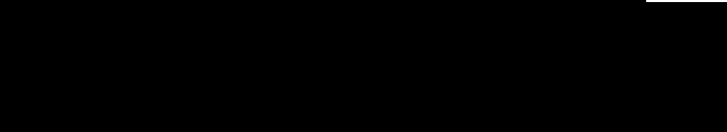
\includegraphics[width=0.9\textwidth]{pictures/primary}
\end{figure}

Natürlich kann jede der Vor- und Nachmethoden vorhanden sein oder nicht. Was zwingend vorhanden sein muss, ist eine anwendbare Primärmethode. Außerdem haben Vor- und Nachmethoden weder Wissen von, noch Einfluss auf das Ergebnis der Primärmethode. Sie eignen sich daher nur für Seiteneffekte. Dafür bieten sie der Klasse, die später erweitert wird, eine Möglichkeit, sicherzustellen, dass eine bestimmte Operation garantiert in allen Subklassen ausgeführt wird. Das kann zum Beispiel bei einer Methode zum Malen eines Bildes das Erstellen der Leinwand sein.

Zusätzlich zu Vor- und Nachmethoden gibt es noch redefinierende Methoden. Sie bestimmen selbst, ob und an welcher Stelle in ihrem Rumpf mit \texttt{call-next-method} (das CLOS-Äquivalent zu super) die nächste Methode aufgerufen werden soll. Die Aufrufreihenfolge ist wie folgt (vgl. \cite[S.103]{keene}):
\begin{itemize}
 \item CLOS ruft die spezifischste redefinierende Methode auf. Sie erhält die gleichen Parameter wie die generische Funktion bzw. Primärmethode.
 \item Falls eine redefinierende Methode \texttt{call-next-method} aufruft:
 \begin{itemize}
  \item Wenn es weitere anwendbare redefinierende Methoden gibt, wird die nächstspezifischste aufgerufen und das Ergebnis zurückgegeben.
  \item Ansonsten wird das komplette Framework aus Vor-, Primär- und Nachmethoden aufgerufen und das Ergebnis zurückgegeben.
 \end{itemize}
\end{itemize}

Es lässt sich eine Klasse Nightowl definieren, die den Rückgabewert der Primärmethode verändert:

\begin{lstlisting}
(defclass Nightowl (Trainer))

(defmethod daily-routine :around ((n Nightowl))
  (display "He slept through the whole day.\n")
  (list (call-next-method) 42))
  
> (daily-routine (make Nightowl))
\end{lstlisting}
{\routput He slept through the whole day.\\
\phantom{.}He walked out.\\
\phantom{.}He caught some Pokemon.\\
\phantom{.}He walked back home.\\
\phantom{.}(\#<void> 42)}

Da redefinierende Methoden entscheiden können, \texttt{call-next-method} nicht aufzurufen, können sie den Aufruf aller Vor-, Nach- und Primärmethoden verhindern. Eine redefinierende Methode muss auch nicht das Ergebnis der Primärmethode zurückgeben. Ein Beispiel ist die folgende Klasse Lazybum:

\begin{lstlisting}
(defclass Lazybum (Trainer))

(defmethod daily-routine :around ((l Lazybum))
  (display "And that was it.\n"))
  
> (daily-routine (make Lazybum))
\end{lstlisting}
{\routput And that was it.}

Die redefinierende Methode verhindert alle weiteren Methodenaufrufe. 

Bei mehreren Oberklassen beziehen sich die ``nächstspezifischste redefinierende Methode'' und ``alle Vor- beziehungsweise Nachmethoden'' auf den kompletten Vererbungsbaum. Es ist möglich eine Klasse Lazyowl zu definieren, die sowohl von Nightowl als auch von Lazybum erbt:

\begin{lstlisting}
(defclass Lazyowl (Nightowl Lazybum))

> (daily-routine (make Lazyowl))
\end{lstlisting}
{\routput He slept through the whole day.\\
\phantom{.}And that was it.\\
\phantom{.}(\#<void> 42)}

Ein Aufruf von \texttt{daily-routine} zeigt, dass die redefinierende Methoden beider Oberklassen aufgerufen werden. 

Im Gegensatz zu Racket sind Ergänzungsmethoden jedoch nicht kompatibel mit Methodenkombination: Sobald eine Kombination in der generischen Funktion für die Methode angegeben wird, führt der Versuch der Definition einer Ergänzungsmethode zu einem Fehler:

\begin{lstlisting}
(defgeneric daily-routine ((t Trainer))
  :combination generic-list-combination)
  
> (daily-routine (make Trainer))
\end{lstlisting}
{\routput He walked out.}

\vspace{-0.3cm}
{\rerror swindle/clos.rkt: arity mismatch; the expected number of arguments does not match the given number; expected: 2; given: 1.}

Ergänzungsmethoden sind lediglich Bestandteil der \emph{standard method combination}, also derjenigen Kombination, die ausgeführt wird, wenn keine andere Methodenkombination angegeben wurde. Sobald eine Kombination angegeben wird, ersetzt diese die \textit{standard method combination} und ein Benutzen von \texttt{:before}, \texttt{:after} und \texttt{:around} führt zu einem Fehler.

Eine Ausnahme von dieser Regel sind redefinierende Methoden, die \texttt{call-next-method} nicht aufrufen; sie sind auch in der Lage, Methodenkombination zu verhindern.

% \subsection{Ergänzungmethoden und Methodenkombination}
% Ergänzungsmethoden sind in CLOS Teil der Standard-Method-Combination (SMC), also der Methodenkombination, die ausgeführt wird, wenn wir nichts anderes angeben. Sobald wir in einer generischen Funktion eine Kombinationsart für die Methode angeben, ist es nicht mehr möglich, auch Ergänzungsmethoden für diese Methode zu definieren.
% 
% Warum ist das so?
% 
% Nehmen wir beispielsweise die \texttt{attack}-Methode aus dem Pokemonbeispiel und nehmen wir außerdem an, dass alle drei Klassen Element, Animal und Pokemon eine Around-Methode definiert haben (Abb. \ref{problem}). Die Methodenkombination sagt uns, wir müssen sowohl die Methode in Element als auch die in Animal auswerten. Pokemon besitzt jedoch eine Around-Methode, die laut SMC zuallererst ausgewertet werden müsste. Welche Regel soll zuerst befolgt werden?
% 
% \begin{figure}[h]
%  \centering
%  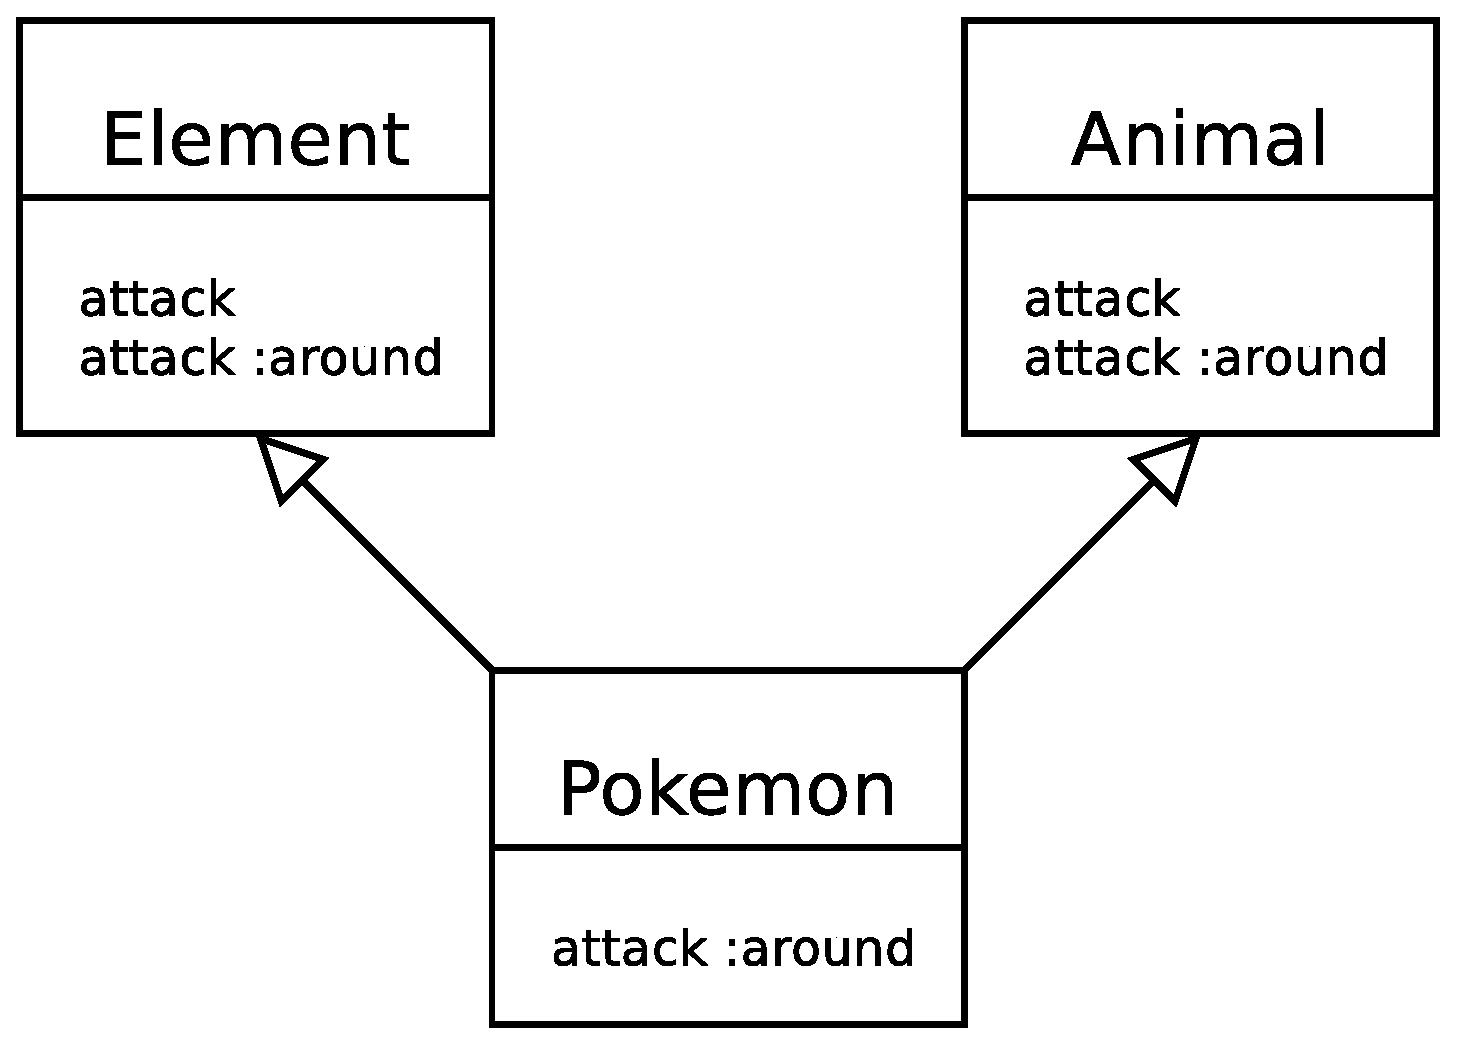
\includegraphics[scale=0.3]{pictures/problem}
%  \caption{Beispiel für Methodenkombination und Ergänzungmethoden.}
%  \label{problem}
% \end{figure}
% 
% Die naheliegende Lösung ist, den Regeln der Standard-Methodenkombination  Vorrang zu geben: wir lassen das Auswertungsschema undverändert, aber anstatt nur einer Primärmethode werten wir alle anwendbaren Primärmethoden aus und kombinieren das Ergebnis.
% 
% Zuallererst muss also die Around-Methode von Pokemon ausgewertet werden. Nehmen wir weiterhin an, die Around-Methode ruft die Methode der Superklasse auf, die spezifischste sei hier die von Element und diese ruft nicht \texttt{call-next-method} auf. Für die Listen-Kombination müssen wir jedoch die primäre Methode von Animal auswerten, die unter Umständen ohne ohne Around-Methode überhaupt keinen Sinn ergibt, zum Beispiel wenn die Around-Methode die Datei öffnet und schließt, die in der primären Methode gelesen wird.
% 
% Man müsste also alle Around-Methoden ausführen, unabhängig davon, ob \texttt{call-next-} \texttt{method} aufgerufen wurde oder nicht. Das steht jedoch in Widerspruch zu der Fähigkeit von Around-Methoden, die Auswertung anderer Methoden verhindern zu können. Die Verbindung von Methodenkombination und dem Überschreiben von Methoden scheint nicht sinnvoll. 
% 
% Vor- und Nachmethoden sind weniger problematisch, denn ihre Auswertungsreihenfolge hängt nicht von ihrem Inhalt ab. Es ist dann vermutlich

Es wurde veranschaulicht, dass ein Umgang mit Mehrfachvererbung in CLOS sehr intuitiv und einfach bereitgestellt wird.

\section{Zwischenfazit}
Das Objektsystem von Racket bietet zwar Mixins und Traits, beide sind jedoch geschickt verpackte Einfachvererbung und werden sehr kompliziert, wenn die Anzahl an Klassen steigt und gleichbenannte Methoden und Felder vorkommen. CLOS hingegen bietet einen sehr intuitiven Umgang mit Mehrfachvererbung. Es ermöglicht generische Methoden, Methodenkombination und Ergänzungsmethoden.
\chapter{Entwurf} 
Das Objektsystem von Racket soll um die Features Mehrfachvererbung, generische Methoden und Ergänzungsmethoden erweitert werden. 

\section{Anforderungen}
Es sollen dabei folgende Anforderungen beachtet werden:
\begin{enumerate}
 \item Bestehender Code in Object-Racket funktioniert genauso wie vorher. Die Erweiterung soll keinen Einfluss auf bestehenden Racket-Code haben. Alle Funktionalität, die das Objektsystem zur Zeit bietet, soll auch nach Hinzufügen der Features auf dieselbe Art funktionieren und das gleiche Ergebnis liefern.
 \item Die Syntax passt sich in das Objektsystem von Racket ein. Neu hinzugefügte Makros und Funktionen sollen konsistent mit bestehenden Makros und Funktionen benannt werden und auf die gleiche Art und Weise aufrufbar sein. 
 \item Die Benutzung ist für jemanden, der CLOS kennt, intuitiv. Die definierten Makros und Funktionen sollen möglichst ähnlich zu benutzen sein wie in CLOS und das gleiche Verhalten zeigen (unter Beachtung von 2.).
\end{enumerate}

Die erste Anforderung soll gewährleisten, dass das Makro auch in bestehenden Racket-Projekten eingebunden werden kann, ohne dass das die Funktionalität bestehender Klassen und Objekte beeinflusst. Die Erweiterung soll dazu ermuntern, Mehrfachvererbung zu nutzen an den Stellen, so es sinnvoll ist und das mit dem geringstmöglichen Änderungsaufwand. Es soll niemand gezwungen sein, alle bestehenden Klassen umzuschreiben, nur damit eine einzelne Klasse Mehrfachvererbung nutzen kann.

Die zweie Anforderung knüpft direkt an die erste an: Es ist einfacher, neue Funktionalität zu benutzen, wenn sie sehr ähnlich zu bereits bestehenden Konzepten ist. Für einen Entwickler, der sich bereits mit dem Objektsystem von Racket auskennt, soll die neue Funktionalität so intuitiv wie möglich sein. Dafür ist es ist beispielsweise hilfreich, wenn generische Funktionenen, die vom Konzept her sehr verwandt zu Methoden sind, auf eine ähnliche Weise benutzt werden können.

Die dritte Anforderung ist interessant für diejenigen, die beide Welten kennen: die von Racket und die von CLOS. Die Erweiterung integriert Bestandteile von CLOS in das Objektsystem von Racket. Dann sollten diese Bestandteile für jemanden, der CLOS kennt, leicht verständlich und möglichst ähnlich zu benutzen sein.

\section{Gewünschtes Verhalten}

\subsection{Mehrere Superklassen}
Für Mehrfachvererbung muss es zunächst möglich sein, mehrere Superklassen anzugeben. Analog zu CLOS soll dies in einer Liste möglich sein. Die Spezifikation der Superklassen als Liste ist jedoch lediglich eine Alternative, die direkte Angabe der Superklasse soll weiterhin möglich sein. Wie in CLOS soll auch eine leere Liste angegeben werden können, in dem Fall wird automatisch die Rootklasse als Superklasse gesetzt. Die folgenden drei Aufrufe sollen zukünftig alle eine Klasse erzeugen, die \texttt{object\%} als (einzige) Superklasse hat (bisher ist in Racket nur die erste Form möglich):

\begin{lstlisting}
(class object% (super-new))
(class () (super-new))
(class (object%) (super-new))
\end{lstlisting}

In der Liste sollen auch mehrere Klassen angegeben werden können. Die Superklassen werden nach ihrer Präzedenz geordnet angegeben; diejenige mit der höchsten Präzedenz kommt zuerst, diejenige mit der niedrigsten Präzedenz zuletzt. 

\begin{lstlisting}
(class (my-class my-other-class ...) (super-new)) 
\end{lstlisting}

Die Funktion \texttt{super-new} sorgt dann dafür, dass die Konstruktoren aller angegebenen  Superklassen aufgerufen werden. Es soll weiterhin an jeder Stelle in Rumpf der Klasse angegeben werden können. 

Gegebenenfalls ist auch eine alternative Definition mit Klassenparameter sinnvoll, sodass der Benutzer Kontrolle darüber hat, in welcher Reihenfolge die Konstruktoren der Superklasse aufgerufen werden. Dann muss jedoch auch mit dem Fall, dass der Benutzer nicht alle Superklassen aufruft, umgegangen werden -- beispielsweise durch Werfen eines Fehlers zur Auswertung oder beim Erstellen eines Objektes, oder durch automatisches Aufrufen aller fehlenden Superklassen am Ende des Rumpfes. Zudem muss abgewogen werden, ob diese Freiheit für den Benutzer die Implementation nicht zu stark verkompliziert.

Falls mehr als eine Superklasse angegeben wird, so erbt die Klasse alle Felder und Methoden der beiden Oberklassen. Gibt es gleichbenannte Felder, so werden im Standardfall die Felder beziehungsweise Methoden der Klasse mit der höheren Präzedenz geerbt.

\subsection{Generische Funktionen}
Da Methoden im Objektsystem von Racket innerhalb von Klassen definiert werden, soll das auch für generische Funktionen gelten. Sie werden in der entsprechenden Oberklasse definiert. Für das attack-Beispiel aus der Racketeinführung wäre das die Klasse Thing, es kann jedoch im Zweifel auch die Klasse \texttt{object\%} erweitert werden. Methodendefinitionen starten in Racket mit \texttt{define/}, daher sollen generische Funktionen mit dem Schlüsselwort \texttt{define/generic} definiert werden. Die Syntax ist wie folgt:

\texttt{(define/generic ({\textless}function-name{\textgreater} {\textless}args{\textgreater}) {\textless}combination{\textgreater})}

Der Objekt-Parameter entfällt. Subklassen können (müssen aber nicht) die generische Funktion durch eine öffentliche Methode implementieren. Für Klassen, die die Methode nicht explizit definieren, wird die Methode durch Methodenkombination erzeugt. Falls die Methodenkombination wegen fehlender Methoden fehlschlägt, gibt es wie in CLOS einen Laufzeitfehler.

Die in CLOS definierten Standardkombinationen sollen auch in Racket möglich sein: \texttt{+, min, max, list, append, begin, and, or}. 
Zusätzlich soll es möglich sein, eigene Kombinationen zu definieren.


\subsection{Vor- und Nachmethoden}
Vor- und Nachmethoden (und ggf. auch Around-Methoden) sollen auf ähnliche Weise über \texttt{define/before}, \texttt{define/after} beziehungsweise \texttt{define/around} definierbar sein. 

\texttt{(define/before ({\textless}method-name{\textgreater} {\textless}args{\textgreater}) {\textless}body{\textgreater})}\\
\texttt{(define/after ({\textless}method-name{\textgreater} {\textless}args{\textgreater}) {\textless}body{\textgreater})}\\
\texttt{(define/around ({\textless}method-name{\textgreater} {\textless}args{\textgreater}) {\textless}body{\textgreater})}

Der Methodenname muss mit einer in der Klasse sichtbaren Primärmethode übereinstimmen. Falls die Klasse keine entsprechende Primärmethode definiert oder erbt, so gibt es einen Laufzeitfehler.
\chapter{Analyse der Implementationsdetails von CLOS}
Um die Konzepte von CLOS auf ein anderes Objektsystem anwenden zu können, ist es notwendig zu verstehen, wie CLOS funktioniert. Wir wollen deshalb einen Blick hinter die Kulissen werfen, die relevanten Konzepte der Implementation aufzeigen und evaluieren, ob sie sich auch auf Racket anwenden lassen.

Makros sind das Sprachmittel, mit dem die Syntax einer Programmiersprache geschrieben und verändert wird. Der Einstiegspunkt einer jeden Erweiterung der Sprache ist ein Makro, das gilt sowohl für die Implementation von CLOS als auch die Erweiterung, die im Rahmen dieser Arbeit entstehen soll. Deshalb soll zunächst kurz auf die Grundlagen von Makros eingegangen werden. Wir betrachten dafür das Makrosystem von Racket. Dieser Teil basiert auf dem Guide ``Fear of Macros'' von Greg Hendershott \cite{fearofmacros} und dem Racket-Guide für Makros \cite{racketguide-macros}.

Anschließend schauen wir uns an, wie CLOS implementiert ist. CLOS ist dabei nicht nur ein Ratgeber zur Implementation von Mehrfachvererbung. Es gibt uns außerdem einen Einblick, wie eine bestehende Sprache mithilfe von Makros und Metaobjekten um ein Objektsystem erweitert werden kann -- eine wichtige Grundlage für die Erweiterung von Racket. Die Implementationsdetails von CLOS sind dem Buch ``The Art of the Metaobject Protocol'' (AMOP) \cite{amop} entnommen. Die CLOS-Implementation in AMOP ist nicht in Racket, sondern Common Lisp und die Quelltextbeispiele wurden unverändert übernommen. Es wird daher zu leichten Abweichungen zu der bisher eingeführten Syntax von Racket oder Makros kommen; die grundlegende Funktionalität ist jedoch die gleiche.

\section{Makros} 
\label{makros}
% \subsection{Transformers}

Ein Makro ist im Grunde eine Funktion. Sie erhält ein Stück Syntax als Eingabe und gibt ein anderes Stück Syntax zurück. Sie \textit{transformiert} Syntax. Wir können einen solchen Syntax-Transformer mit \texttt{define-syntax} definieren:

\begin{lstlisting}
(define-syntax foo
  (lambda (stx)
    (syntax "I am foo")))
\end{lstlisting}

Ein Aufruf von foo ergibt dann:

\begin{lstlisting}
> (foo)
\end{lstlisting}
{\routput {\qq}I am foo{\qq}}

Durch die Verwendung von \texttt{define-syntax} geschieht eine Transformer-Bindung. Wir teilen dem Racket-Compiler mit: ``Wann immer du im Quelltext ein Stück Syntax findest, das mit \texttt{foo} startet, gib es an meine Transformer-Funktion und ersetze es mit der Syntax, die ich dir zurück gebe.'' Racket gibt also alles, das aussieht wie \texttt{(foo ...)} an unsere Funktion und wir können neue Syntax zurückgeben, die stattdessen verwendet wird, ähnlich zu einer Suchen-und-Ersetzen-Operation.

\begin{lstlisting}
> (foo 1 2 3)
\end{lstlisting}
{\routput ``I am foo''}

Die Transformation passiert rein auf Syntax-Ebene. Erst \textit{nachdem} die Syntax ersetzt wurde, geschieht die Auswertung. Wir könnten Anstelle der 1 auch eine Division durch 0 schreiben und es würde keinen Fehler geben, da die Parameter von \texttt{foo} nach der Transformation nicht mehr Teil der Syntax sind.

% \subsection{Syntax-Objekte}
Übsicherweise soll die Eingabe-Syntax transformiert werden. Wenn wir Syntax definieren, erhalten wir ein Syntax-Objekt:

\begin{lstlisting}
(syntax (+ 1 (* 2 3)))
\end{lstlisting}
{\routput\#<syntax:2:14 (+ 1 (* 2 3))>}

Ein Syntaxobjekt besteht aus einer Repräsentation des Ausdrucks, enthält aber auch Informationen über die Datei, Zeile und Spalte in der es definiert wurde sowie den Sichtbarkeitsbereich von Variablen (\emph{lexical scope}). All diese Informationen kann man mit entsprechenden Funktionen abfragen.

Beim Transformieren von Syntax nehmen wir üblicherweise die Bestandteile der Syntax, die uns gegeben wird, ändern ihre Reihenfolge, ersetzen einige von ihnen oder führen gänzlich neue Bestandteile ein.

Ein simples Beispiel, das die Reihenfolge der Syntax umkehrt:

\begin{lstlisting}
(define-syntax (reverse-me stx)
  (datum->syntax stx (reverse (cdr (syntax->datum stx)))))
  
> (reverse-me "backwards" "am" "I" values)
\end{lstlisting}
{\routput {\qq}I{\qq} {\qq}am{\qq} {\qq}backwards{\qq}}

Die Syntax

\begin{lstlisting}
#'(reverse-me "backwards" "am" "I" values)
\end{lstlisting}

(die Raute ist eine Kurzform für \texttt{syntax}) wird zunächst mit \texttt{syntax->datum} in den quotierten Ausdruck 

\begin{lstlisting}
'(reverse-me "backwards" "am" "I" values)
\end{lstlisting}


umgewandelt. Nachdem der Name der Funktion, \texttt{reverse-me}, abgeschnitten wurde, werden die Wörter mit \texttt{reverse} in umgekehrte Reihenfolge gebracht

\begin{lstlisting}
'(values "I" "am" "backwards")
\end{lstlisting}

und anschließend die Liste wieder in Syntax umgewandelt. Diese Syntax wird vom Compiler ausgewertet und ergibt schließlich die oben genannte Ausgabe.


Der Syntax-Transformer wird zur Übersetzungszeit ausgewertet. Das bedeutet, dass die Teilstücke der Syntax zwar verschoben und ersetzt werden -- aber nicht ausgewertet. Das geschieht erst zur Laufzeit. Dadurch ermöglichen uns Makros beispielsweise die Definition eines eigenen \texttt{if} durch Benutzen von \texttt{cond}.

Würden wir \texttt{if} als normale Racket-Funtion definieren, so würden alle Parameter ausgewertet, bevor sie überhaupt an die Funktion gegeben werden. Das wird spätestens dann sichtbar, wenn sie Seiteneffekte beinhalten oder in einem Zweig der Fallunterscheidung ein rekursiver Aufruf steckt. Durch die Definition als Makro haben wir die Möglichkeit das \texttt{if} bereits zur Übersetzungszeit durch ein \texttt{cond} zu ersetzten.


Eine Liste immer mit \texttt{car}, \texttt{cadr} und so weiter zu zerlegen ist jedoch sehr anstrengend und fehleranfällig. Eleganter geht es mithilfe von Pattern-Matching. %Racket bietet dafür die Funktion \texttt{match}. 


% \subsection{Pattern Matching}
Das Makrosystem von Racket bietet eine sehr bequeme Funktion für Pattern Matching: \texttt{syntax-case} und dessen Kurzform \texttt{define-syntax-rule}. Anstatt die Syntax per Hand auseinanderzunehmen, stellen wir ein Template bereit, welches Variablen aus dem Pattern nutzt.

\begin{lstlisting}
(define-syntax-rule 
  (my-if-using-syntax-rule condition true-expr false-expr) ; Pattern
  (cond [condition true-expr]                              ; Template
        [else false-expr]))
\end{lstlisting}

Diese Definition sieht so einfach aus, dass man denken könnte, es wäre eine normale Laufzeit-Funktion -- aber sie ist es nicht. Sie läuft zur Übersetzungszeit. 


\texttt{define-syntax-rule} bindet ein Makro, das ein einzelnes Pattern abgleicht. Rackets Makro-System unterstützt mit \texttt{syntax-rules} jedoch auch Transformer für mehrere Patterns, die mit dem gleichen Bezeichner starten.

Beispielsweise könnten wir ein Makro definieren, das sowohl zwei als auch drei Werte miteinander vertauschen kann (nach \cite{racketguide-macros}):

\begin{lstlisting}
(define-syntax rotate
  (syntax-rules ()
    [(rotate a b) (swap a b)]
    [(rotate a b c) (begin
                     (swap a b)
                     (swap b c))]))
\end{lstlisting}

Es ist sogar möglich, Patterns beliebiger Länge in einem Makro zu matchen. Für eine beliebige Anzahl an Parametern gibt es die ``\texttt{...}``-Schreibweise. Das Makro ähnelt dann einer rekursiven Funktion mit einem Standardfall (oder mehr) und einer Regel, wie mit dem Rest der Parameter zu verfahren ist (nach \cite{racketguide-macros}):

\begin{lstlisting}
(define-syntax rotate
  (syntax-rules ()
    [(rotate a) (void)]
    [(rotate a b c ...) (begin
                          (swap a b)
                          (rotate b c ...))]))
\end{lstlisting}

Mit \texttt{syntax-rules} lässt sich recht leicht ein Makro schreiben, das  \texttt{my-class}-Aufrufe matcht, dabei mehrere Superklassen akzeptiert, von uns gewünschte Funktionalität ausführt und anschließend das \texttt{class}-Makro von Racket mit selbst definierten Klassenoptionen aufruft.


\section{Grundstruktur von CLOS}
Es gibt drei Schlüsselwörter, die die Objektstruktur von CLOS definieren:  \texttt{defclass}, \texttt{defgeneric} und \texttt{defmethod}. Implementiert sind sie als Makros, die die interne Repräsentation der Klassen, generischen Funktionen und Methoden erzeugen und damit die Übersicht über die Informationen behalten, die in ihren Definitionen angegeben wurden.

Das \texttt{defclass}-Makro expandiert beispielsweise zu einem internen Methodenaufruf. Es werden die angegebenen Superklassen, Slots und anderen Optionen übergeben und die Methode sorgt dafür, dass eine interne Repräsentation dieser Klasse erstellt wird und anschließend das Klassenobjekt zurückgegeben wird.

Die Informationen werden in Form von Objekten festgehalten -- internen Objekten, die der Nutzer niemals zu sehen bekommt. Diese Objekte werden daher ``Metaobjekte'' genannt.

Es entsteht eine Struktur in drei Schichten:
\begin{itemize}
 \item die Makro-Expansions-Schicht: eine dünne Schicht, die die wenigen syntaktischen Konstrukte bereitstellt, die der Nutzer zu sehen bekommt, wie das \texttt{defclass}-Makro.
 \item Die ``Leim''-Schicht: hier werden die externen Namen auf die intern benutzten Metaobjekte abgebildet, zum Beispiel die Funktion \texttt{find-class}, welche ein Metaobjekt anhand des Namens heraussucht.
 \item Die Support-Schicht: Hier ist das Verhalten von Klassen, Instanzen, generischen Funktionen und Methoden implementiert. Das Metaobjekt-Protokoll konzentriert sich hauptsächlich auf diese Schicht.
\end{itemize}

Wir werden untersuchen, ob ein analoges Vorgehen auch für die Implementation von Mehrfachvererbung in Racket möglich ist. Um diese Struktur zu verstehen, wollen wir daher die einzelnen Schichten genauer betrachten. Wir fangen mit der untersten Schicht an: bei den Metaobjekten.

\section{Metaobjekte}
CLOS ist zirkulär definiert: Der Code, der CLOS implementiert, benutzt CLOS-Klassen und -Objekte. CLOS hat Wege gefunden, diese Zirkularität zu umgehen, über Bootstrapping und Reflection, aber das zu verstehen ist nicht Bestandteil dieser Arbeit. 

Wir wollen später ein bereits fertig definiertes Objektsystem verwenden, um darauf aufbauend ein mächtigeres Objektsystem zu definieren, das Objektsystem von Racket. Mit einer etwas anderen Sichtweise bietet die CLOS-Implementation uns genau das: es wird ein Objektsystem verwendet, um das Verhalten eines anderen Objektsystems zu definieren. Das erste Objektsystem besteht aus den intern benutzten Klassen und Objekten, das zweite aus den externen Klassen und Objekten, die dem Anwender bereitgestellt werden.

Es gibt in CLOS also interne Objekte, die das Verhalten der dem Benutzer sichtbaren Klassen und Objekte definieren. Objekte über andere Objekte -- Metaobjekte. Es gibt solche Metaobjekte für alle Konstrukte, die für den Benutzer definiert werden sollen und über die daher Informationen gesammelt werden müssen: Klassenmetaobjekte für Klassen, Generische-Funktionen-Metaobjekte für generische Funktionen und Methodenmetaobjekte für Methoden. 

Wo es Objekte gibt, muss es auch eine Klasse geben, die ihr Verhalten definiert. Die Klasse, die das Verhalten von Metaobjekten definiert, wird Metaklasse genannt. 

Klassen-Metaobjekte sammeln beispielsweise all diejenigen Information, die zur Erstellung der aktuellen und zukünftiger Klassen relevant sind: den Namen der Klasse, die angegebenen Superklassen, definierte Slots, geerbte Slots, die Klassenpräzedenzliste, die direkten Subklassen und die definierten Methoden. 

Die ``Klassen-Metaklasse'' ist dann lediglich die Beschreibung, wie die Metaobjekte aussehen. Es ist eine ganz normale CLOS-Klasse, mit dem einzigen Unterschied, dass sie nur intern verwendet wird:

\begin{lstlisting}
(defclass standard-class ()
  ((name :initarg :name
         :accessor class-name)
   (direct-superclasses :init-arg :direct-superclasses
                        :accessor class-direct-superclasses)
   (direct-slots :accessor class-direct-slots)
   (class-precedence-list :accessor class-precedence-list)
   (effective-slots :accessor class-slots)
   (direct-subclasses :initform ()
                      :accessor class-direct-subclasses)
   (direct-methods :initform ()
                   :accessor class-direct-methods)))
\end{lstlisting}

Das \texttt{defclass}-Makro parst die Klassendefinition und verwandelt sie in einen Aufruf an die Methode \texttt{ensure-class} aus der ``Leim''-Schicht. 

\begin{lstlisting}
(defmacro defclass (name direct-superclasses direct-slots &rest options)
  ´(ensure-class ',name
    :direct-superclasses ,(canonicalize-direct-superclasses 
                            direct-superclasses)
    :direct-slots ,(canonicalize-direct-slots direct-slots)
    ,@(canonicalize-defclass-options options)))
\end{lstlisting}

Der Makro-Befehl ist sehr ähnlich zu \texttt{define-syntaxrule}: das Pattern mit Name, Superklassen, Slots und anderen Optionen wird gematcht und im anschließenden Template benutzt -- einem Aufruf der Methode ensure-class. Die \texttt{canonicalize}-Funktionen übernehmen die weitere Makro-Expansion, wie das Auswerten der Slot-Optionen, das Expandieren von Accessor-Optionen zu den Reader und Writer, Ersetzen der Namen der Superklassen durch die zugehören Metaobjekte und so weiter. Sie tun praktisch ``die ganze Arbeit'' der Expansion.

\texttt{ensure-class} nimmt dann den Namen und die Argumente der Klasse und definiert ein Klassenobjekt mit dem Namen:

\begin{lstlisting}
(defun ensure-class (name &rest all-keys)
  (if (find-class name nil)
      (error "Can't redefine the class named ~S.", name)
      (let ((class (apply #'make-instance
                          'standard-class :name name all-keys)))
        (setf (find-class name) class)
        class)))
\end{lstlisting}

Es werden die expandierten Klassenoptionen genommen und mit ihnen ein neues Metaobjekt erstellt. Das Metaobjekt wird zur Liste der bekannten Klassen hinzugefügt und anschließend zurückgegeben. 

Es gibt demnach eine Tabelle von Klassen-Metaobjekten, die bereits erstellt wurden, sowie Funktionen zum Abfragen, ob ein Objekt bereits existiert und zum Hinzufügen eines Objekts:

\begin{lstlisting}
(let ((class-table (make-hash-table :test #'eq)))
  
  (defun find-class (symbol &optional (errorp t))
    (let ((class (gethash symbol class-table nil)))
      (if (and (null class) errorp)
          (error "No class named ~S." symbol)
          class)))
  
  (defun (setf find-class) (new-value symbol)
    (setf (gethash symbol class-table) new-value))
)
\end{lstlisting}

\texttt{make-instance} ist eine Methode der untersten Schicht und führt noch einige notwendige Initialisierungen durch, wie das Hinzufügen des Objekts als Subklasse zu seinen Superklassen, Konvertieren der Liste von Sloteigenschaften in tatsächliche Slot-Definitionen oder die Definition von Accessor-Methoden. 

Für eine Implementation von Mehrfachvererbung in Racket brauchen wir ebenfalls Informationen darüber, welche Klassen mit welchen Superklassen, Feldern und Methoden bereits definiert wurden. Die Methodenkombination beispielsweise basiert auf den Ergebnissen aller Methoden in allen Superklassen -- nach dieser Information können wir ein Klassenobjekt nach der Erstellung durch Racket jedoch nicht mehr fragen; in ihm existiert jede Methode nur genau einmal.

Anstelle von CLOS-Metaobjekten über CLOS-Klassen wollen wir also Racket-Metaobjekte über Racket-Klassen erstellen. Um Mehrfachvererbung und Methodenkombination zu implementieren, müssen wir wissen, in welcher Vererbungshierarchie die Klassen stehen und welche Felder und Methoden sie definieren. Das sind genau die Informationen, die sich auch das Metaobjekt in CLOS merkt:

\begin{tabular}{p{5cm}p{9cm}}
 \texttt{direct-superclasses} & Die Liste der direkten Superklassen. \\
 \texttt{direct-slots} & Die Felder, die die Klasse definiert. \\
 \texttt{class-precedence-list} & Die Reihenfolge, in der von den Superklassen geerbt wird.\\
 \texttt{effective-slots} & Die Ergänzung von \texttt{direct-slots} um die geerbten Felder. \\
 \texttt{direct-methods} & Die Methoden, die die Klasse definiert.
\end{tabular}

Da Racket-Klassen nicht benannt sind, entfällt das Feld für den Namen. Um die Metaobjekte für Testzwecke unterscheiden zu können, bietet es sich jedoch gegebenenfalls an, sie zu nummerieren. Die Information über die Subklassen einer Klasse wird in CLOS hauptsächlich für spätere Verwendung durch den Benutzer bereitgestellt, sie ist nicht notwendig für die Umsetzung von Mehrfachbererbung. 

Analog zu CLOS muss es dann auch eine ``Leim''-Schicht geben, die dafür sorgt, dass die Metaobjekte erstellt und verwaltet werden. Da Racket-Klassen nicht benannt sind, wird selbst bei identischer Klassendefinition immer eine neue Klasse erzeugt; der Test auf Enthaltensein in der Liste der bereits erzeugten Klassen entfällt demnach.

\section{Klassenpräzedenz}
Wir haben fast alle Schritte gesehen, die mit dem Erstellen eines Klassen-Metaobjekts zu tun haben: von \texttt{defclass} über \texttt{ensure-class} bis hin zu \texttt{make-instance}. Die verbleibenden Schritte haben mit Vererbung zu tun:
\begin{itemize}
 \item Berechnen und Speichern der Klassenpräzedenzliste.
 \item Berechnen und Speichern der vollständigen Menge von Slots, bestehend aus direkt in der Klasse definierten und von Superklassen geerbten Slots.
\end{itemize}

Auch für Racket-Objekte müssen wir diese Berechnungen durchführen.

In CLOS führt die Methode \texttt{finalize-inheritance}, die von \texttt{make-instance} aufgerufen wird, beide Schritte aus:

\begin{lstlisting}
(defun finalize-inheritance (class)
  (setf (class-precedence-list class)
        (compute-class-precedence-list class))
  (setf (class-slots class)
        (compute-slots class))
  (values))
\end{lstlisting}

Die Klassenpräzedenzliste (nach \cite[S. 118ff]{keene}) beinhaltet die Klasse selbst und all ihre Superklassen, ohne Duplikate. Die Reihenfolge der Klassen ist dabei relevant; sie sind von der spezifischsten zur am wenigsten spezifischen Klasse geordnet. Wenn eine Klasse spezifischer als eine zweite Klasse ist, so hat sie Präzedenz über die zweite Klasse. Es gibt zwei Regeln, die die Reihenfolge von Klassen in der Präzedenzliste bestimmen:

\begin{enumerate}
 \item Eine Klasse hat immer Präzedenz über ihre Superklassen.
 \item Jede Klassendefinition legt die Präzedenzreihenfolge ihrer direkten Superklassen fest.
\end{enumerate}

Die erste Regel erlaubt es einer Klasse, Verhalten ihrer Superklasse zu überschreiben oder verändern.

Die zweite Regel bewirkt, dass die Reihenfolge direkter Superklassen durch die Reihenfolge der Superklassen im \texttt{defclass}-Makro festgelegt ist. Das heißt, jede angegebene Klasse ist spezifischer als die Klassen, die weiter hinten in der Liste stehen.

Anhand der ersten Regel kennen wir sofort die spezifischste und unspezifischste Klasse jeder Klassenpräzedenzliste. Die Klasse selbst ist die spezifischste und die Wurzelklasse, in Common Lisp \texttt{t} (und noch eine Ebene tiefer \texttt{standard-object}), die unspezifischste in jeder Klassenpräzedenzliste.

Wenn CLOS die Klassenpräzedenzliste einer Klasse bestimmt, startet es bei der Definition der Klasse. Es wendet beide Regeln auf die Klassendefinition an und erhält so eine Liste von Ordnungsconstraints für die direkten Superklassen. Anschließend werden die Regeln auch auf jede direkte Superklasse angewendet, und so weiter, bis alle Pfade in der Wurzelklasse \texttt{t} enden. Das Ergebnis ist eine Menge von Ordnungsconstraints aller beteiligten Klassen.

Der nächste Schritt ist es, eine Sortierung zu finden, die alle Einzelconstraints erfüllt. CLOS führt dazu eine topologische Sortierung durch: das Ermitteln einer Reihenfolge, in der alle Teil-Constraints erfüllt sind. Es entstehen drei Möglichkeiten:
\begin{enumerate}
 \item genau eine Reihenfolge erfüllt alle Constraints
 \item mehrere Reihenfolgen erfüllen alle Constraints
 \item keine Reihenfolge erfüllt alle Constraints
\end{enumerate}

In den ersten beiden Fällen erzeugt CLOS eine Klassenpräzedenzliste. Im dritten Fall wird ein Fehler signalisiert. Für das Pokemon-Beispiel (Abb. \ref{pokemon}) ergeben sich beispielsweise die folgenden Constraints:

\begin{tabular}{l|c}
 \textbf{Constraint} & \textbf{Regel}\\ \hline
 \texttt{Pokemon {\guillemotright} Element} & 1\\
 \texttt{Pokemon {\guillemotright} Animal}  & 1\\
 \texttt{Element {\guillemotright} Animal}  & 2\\
 \texttt{Element {\guillemotright} Thing}   & 1\\
 \texttt{Animal  {\guillemotright} Thing}   & 1
\end{tabular}

Es gibt nur eine totale Ordnung, die alle Constraints erfüllt:

(\texttt{Pokemon Element Animal Thing standard-object t})

Oft ergeben die zwei Präzedenzregeln keine eindeutige Reihenfolge. Nehmen wir zum Beispiel an, Element und Animal haben keine gemeinsame Superklasse, sondern nur Element erbt von Thing und Animal von einer neuen Klasse Creature (Abb. \ref{creature}). 

\begin{figure}[h]
 \centering
 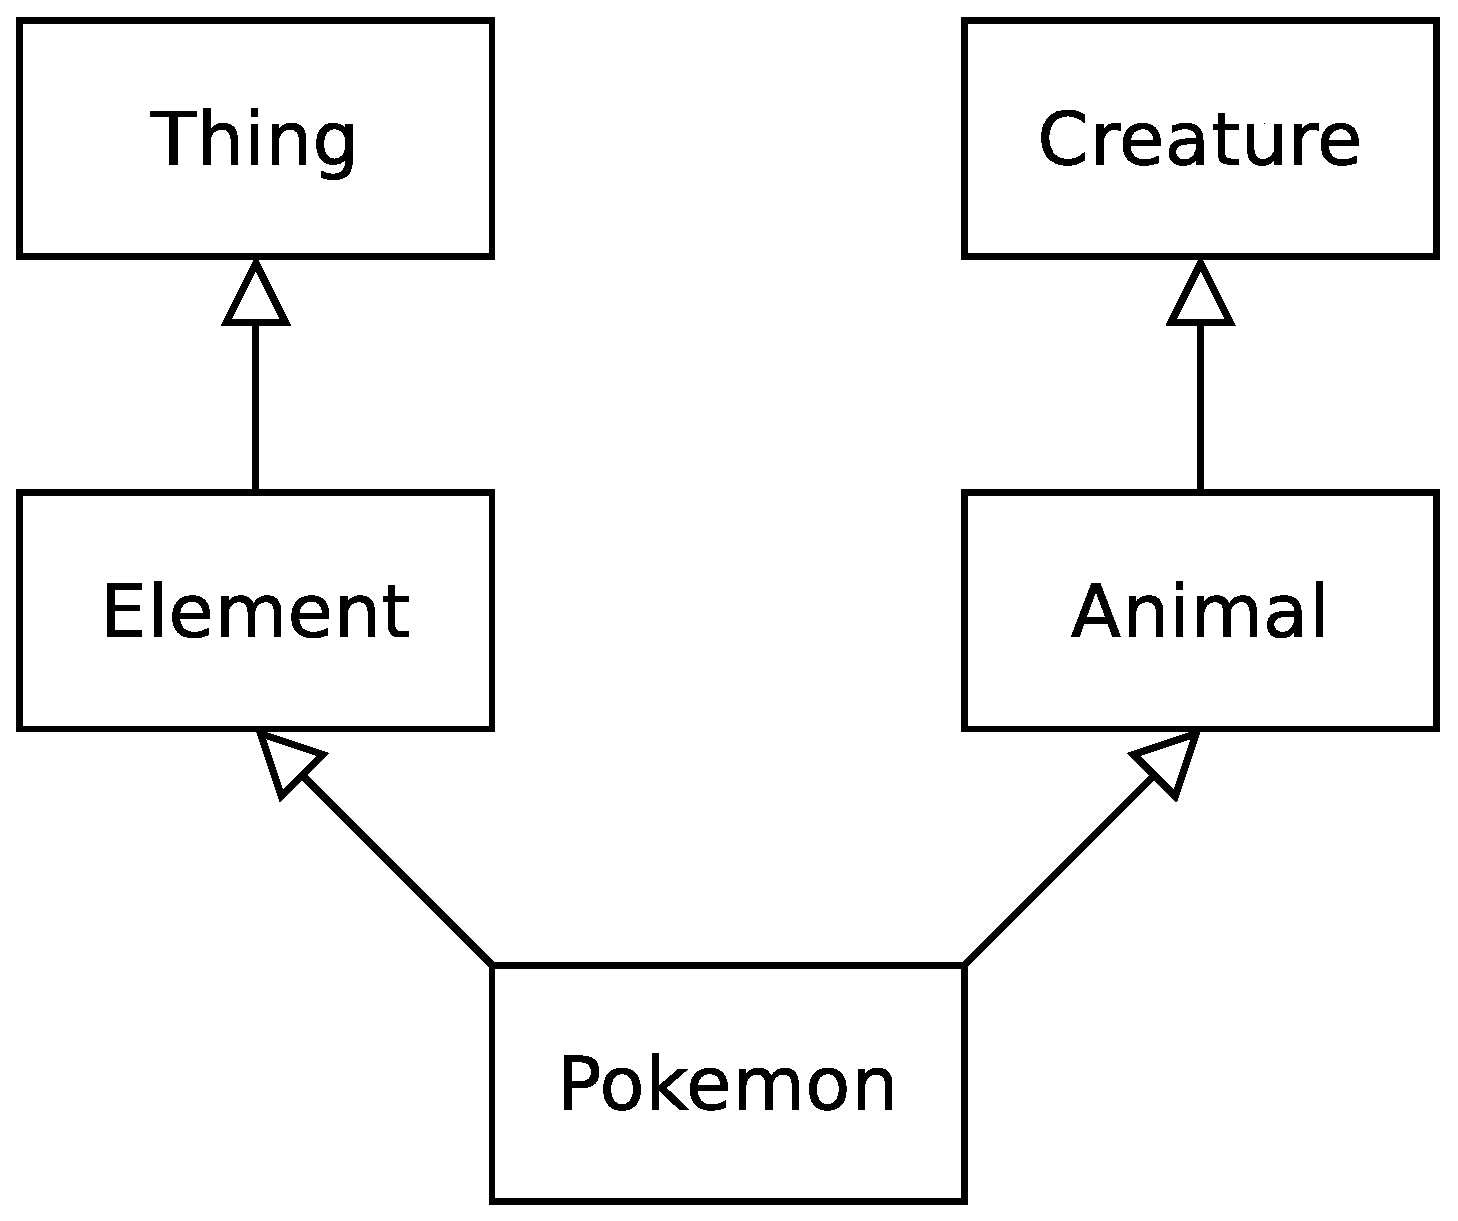
\includegraphics[scale=0.3]{pictures/creature}
 \caption{Vererbungshierarchie mit uneindeutiger Klassenpräzedenz.}
 \label{creature}
\end{figure}

Für Element und Creature sowie Thing und Creature gibt es dann nach den bisher bekannten Regeln kein Constraint, das eine Reihenfolge festlegt. Es ergeben sich drei mögliche Klassenpräzedenzlisten:

(\texttt{Pokemon Element Animal Creature Thing standard-object t})\\
(\texttt{Pokemon Element Animal Thing Creature standard-object t})\\ 
(\texttt{Pokemon Element Thing Animal Creature standard-object t})

CLOS entscheidet sich in dem Fall deterministisch für eine der möglichen Reihenfolgen: diejenige, in der Klassen aus einem Teilbaum möglichst nah beieinander sind. Wenn wir die Klassenhierarchie betrachten, so bilden Element und Thing einen Teilbaum, Animal und Creature einen anderen. CLOS würde demnach die dritte Möglichkeit bevorzugen, in der die Klassen direkt aufeinander folgen.

Falls die Reihenfolge der indirekten Superklassen für das Programm relevant ist, so ist es auch möglich, dies als zusätzliches Constraint anzugeben. Nehmen wir beispielweise an, wir wollen, dass Creature in der Klassenpräzedenzliste vor Thing kommt. Wir können dieses Verhalten erzielen, indem wir die Klassen per Hand zu den ``direkten'' Superklassen in der Klassendefinition von Pokemon hinzufügen:

\begin{lstlisting}
(defclass Pokemon (Element Animal Creature Thing)
  ... )
\end{lstlisting}

Es werden dadurch zwei neue Constraints zur Liste hinzugefügt:

\begin{tabular}{l|c}
 \textbf{Constraint} & \textbf{Regel}\\
 \hline
 \texttt{Animal $>$ Creature} & 2\\
 \texttt{Creature $>$ Thing}  & 2\\
\end{tabular}

Diese zusätzlichen Regeln bewirken, dass es nun nur noch eine mögliche Klassenpräzedenzliste gibt:

(\texttt{Pokemon Element Animal Creature Thing standard-object t})\\

Der Fall, dass keine Reihenfolge alle Constraints erfüllt, tritt auf, wenn zwei Oberklassen gegensätzliche Vererbungsreihenfolgen haben. Das ist zum Beispiel gegeben, wenn wir per Hand eine der Klassen Creature oder Thing vor den Klassen Element und Animal in der Klassendefinition anführen:

\begin{lstlisting}
(defclass Pokemon (Element Creature Animal)
  ... )
\end{lstlisting}

Es ergeben sich dann zwei widersprüchliche Constraints:

\begin{tabular}{l|c}
 \textbf{Constraint} & \textbf{Regel}\\
 \hline
 \texttt{Animal $>$ Creature} & 1\\
 \texttt{Creature $>$ Animal}  & 2\\
\end{tabular}

In dem Fall signalisiert CLOS einen Fehler, da es keine Klassenpräzedenzliste erstellen kann, die konsistent mit allen Constraints ist.

Eine Beispielimplementation des Algorithmus für die Berechnung der Klassenpräzedenzliste kann in \cite[S.24f,291f]{amop} nachgelesen werden. Eine der Anforderungen an die Implementation von Mehrfachbererbung in Racket war, dass sie möglichst ähnlich zu der von CLOS funktionieren soll. Es wird daher die gleiche topologische Sortierung verwendet werden.

CLOS nutzt dann die Klassenpräzedenzliste, um die effektiven Slots zu berechnen:

\begin{lstlisting}
(defun compute-slots (class)
  ... ; conversion to slot object here
  (remove-duplicates
    (apply #'append 
           (mapcar #'class-direct-slots
                   (class-precedence-list class)))
    :key #'slot-definition-name
    :from-end t))
\end{lstlisting}

Es werden die direkten Slots aller Klassen in der Reihenfolge der Präzedenzliste gesammelt und anschließend gleichbenannte Slots entfernt. Dadurch verbleibt nur der Slot der Klasse mit der höchsten Präzedenz in der Liste. Das lässt sich auch leicht auf Definitionen von Racket-Feldern abbilden.

CLOS wandelt die Slot-Definition anschließend noch in Slot-Objekte um. Diese Umwandlung wird Racket für uns übernehmen.

Mit den den CLOS-Konzepten, die wir bisher kennengelernt haben, lässt sich  unser Makro erweitern um Funktionen, die Informationen über die Klasse in Form eines Metaobjektes speichern, die Klassenpräzedenzliste bestimmen und  die effektiven Felder ermitteln. Die Vererbung von Feldern ist damit bereits abgedeckt. Was noch fehlt, ist die Vererbung von Methoden.

\section{Mehrfachvererbung und Methodenkombination}
Analog zu Klassen gibt es auch für Methoden und generische Funktionen Metaobjekte, um eine Übersicht über die relevanten Informationen zu behalten. Eine generische Funktion fasst eine Menge von Methoden mit der gleichen Signatur zusammen und das zugehörige Metaobjekt merkt sich genau diese Dinge: den Namen, die Parameterliste sowie die Methoden, die die generische Funktion implementieren.

\begin{lstlisting}
(defclass standard-generic-function ()
  ((name :initarg :name
         :accessor generic-function-name)
   (lambda-list :initarg :lambda-list
                :accessor generic-function-lambda-list)
   (methods :initform ()
            :accessor generic-function-methods)))
\end{lstlisting}

Die Makros \texttt{defgeneric} und \texttt{defmethod} expandieren dann, analog zu \texttt{defclass}, zu einem Aufruf von \texttt{ensure-generic-function} beziehungsweise \texttt{ensure-method}. \texttt{ensure-generic-function} fügte eine neue generische Funktion zur Liste hinzu während \texttt{ensure-method} die Methode zu einer bestehenden generischen Funktion hinzufügt. Falls es noch keine generische Funktion für die Methode gibt, wird sie erzeugt. In CLOS gibt es zu jeder Methode eine generische Funktion, unabhängig davon, ob der Benutzer sie explizit angibt oder nicht.

Welche Methode bei dem Aufruf einer generischen Funktion ausgeführt wird, hängt von den Argumenten und der Kombinationsart ab. In CLOS ist die Klasse (oder die Klassen), auf die eine Methode spezialisiert ist, Teil der Methodenparameter. 

Falls der Benutzer nichts anderes angibt, geschieht die \emph{standard method combination}, also die Ausführung der spezifischsten Primärmethode und ihrer Ergänzungsmethoden. Sie erfolgt in drei Schritten:
\begin{enumerate}
 \item Bestimmen, welche Methoden anwendbar sind. Methoden sind anwendbar, wenn sie auf die gleiche Klasse wie die auszuführende Methode oder eine ihrer Oberklassen spezialisiert sind.
 \item Sortieren der anwendbaren Methoden nach Präzedenz.
 \item Ausführen der Liste anwendbarer Methoden.
\end{enumerate}

Andere Kombinationsarten werden in AMOP nicht behandelt, aber das gleiche Schema lässt sich sowohl an Ergänzungsmethoden als auch an Methodenkombination anpassen. Sie unterscheiden sich nur darin, welche Methoden anwendbar send, welche Art der Präzedenz für die Sortierung gewählt wird und wie die Methoden anschließend ausgeführt werden (Tabelle \ref{combination}). Falls keine anwendbare Primärmethode gefunden wurde, so wird ein Fehler signalisiert.

\begin{table}[h]
\begin{tabular}{|p{4.7cm}|p{4.5cm}|p{4.5cm}|}
 \hline
 \textbf{Schritt} & \textbf{Ergänzungsmethoden} & \textbf{Methodenkombination}\\\hline
 Bestimmen, welche Methoden anwendbar sind. & Primärmethoden und Ergänzungsmethoden & Primärmethoden \\\hline
 Sortieren der anwendbaren Methoden nach Präzedenz. & Sortieren der Methoden in der Reihenfolge Around, Before, spezifischste Primärmethode, After und innerhalb einer Kategorie nach Klassenpräzedenz & Sortieren der Methoden nach Klassenpräzedenz\\\hline
 Ausführen der Liste anwendbarer Methoden. & Sequentiell & Kombination\\\hline
\end{tabular}
 \caption{Vorgehensweise bei der Methodenkombination.}
 \label{combination}
\end{table}

Auf analoge Weise lässt sich Methodenkombination auch für Racket umsetzen: 
Wir erlauben die Optionen \texttt{define/generic}, \texttt{define/before}, \texttt{define/around} und \texttt{define/after} im \texttt{class}-Makro. Wann immer eine generische Funktion oder Methode angegeben wird, merken wir uns die relevanten Informationen in Form eines Metaobjekts. Und wir sorgen dafür, dass die Methodendefinitionen, für die eine Kombination existiert, durch eine entsprechende Kombinationsmethode ersetzt werden, bevor Racket die Klassendefinition auswertet.

Das ist alles, was wir benötigen.


\chapter{Umsetzung}  
\label{implementation}
Im Rahmen dieser Arbeit ist ein Makro entstanden, das das \texttt{class}-Makro um Mehrfachvererbung und Methodenkombination erweitert. Das Makro nimmt die übergebene Syntax, hält wichtige Informationen in Form von Metaobjekten fest und generiert schließlich die Syntax, die vom eigentlichen \texttt{class}-Makro ausgewertet wird.

\section{eval}

Das erste Problem, das sich dabei stellt ist, dass Racket es nicht erlaubt, mehrere Superklassen anzugeben. Wir können zwar ein Makro schreiben, das mehrere Superklassen akzeptiert, aber der Makroaufruf, zu dem schlussendlich expandiert wird, darf nur eine Superklasse beinhalten. Das bedeutet, wir müssen aus den angegebenen Klassen selbst eine Superklasse erzeugen, die alle Eigenschaften der Klassen in sich vereinigt und diese als offizielle Superklasse angeben. Wie genau das funktioniert, sehen wir später, aber wir werden dafür die Klassenoptionen ebenjener Superklasse zusammenbauen, in einen \texttt{class}-Aufruf stecken und dann auswerten müssen.

Das Problem ist: \texttt{class} ist ein Makro, keine Funktion. Wir können es nicht einfach mit \texttt{apply} auf eine von uns zusammengestellte Liste von Klassenoptionen anwenden. Die andere naheliegende Option ist \texttt{eval}, welche jedoch nicht ohne weiteres außerhalb der Interaktionskonsole benutzt werden kann. Das Bereitstellen von \texttt{eval} auch innerhalb des Definitionsfensters geschieht noch vor der eigentlichen Expansion des Makros, deshalb soll auch hier zuerst darauf eingegangen werden.

\texttt{eval} ist eine Funktion in Racket, die einen quotierten Ausdruck nimmt und ihn auswertet. Salopp gesagt entfernt die Funktion einfach ein Quotierungszeichen (wenn es eins gibt):

\begin{lstlisting}
> (define x 42)
> 'x
\end{lstlisting}
{\rsymbol x}

\begin{lstlisting}
> (eval 'x)
\end{lstlisting}
{\routput 42}

Wir können damit insbesondere einen quotierten Funktionsaufruf auswerten:

\begin{lstlisting}
> (eval '(+ 1 2))
\end{lstlisting}
{\routput 3}

Aber \texttt{eval} funktioniert ohne weiteres nur in der Interaktionskonsole. Versuchen wir im Definitionsfenster den gleichen Ausdruck auszuwerten, so erhalten wir einen Fehler.

{\color{red}\ttfamily\small\hspace{5pt} +: unbound identifier;}\\
{\color{red}\ttfamily\small\hspace{5pt} also, no \#\%app syntax transformer is bound in: +}\\

\texttt{eval} kann die Bindungen des Kontextes, in dem es aufgerufen wird, nicht sehen. Das beinhaltet auch alle importierten Racket-Funktionen, selbst \texttt{+}. Damit \texttt{eval} Zugriff auf die Umgebung hat, in der es aufgerufen wird, muss man einen Namescpace mit übergeben. In der Interaktionskonsole passiert das automatisch; im Definitionsfenster müssen wir es per Hand machen. Dafür kann als zweiter Parameter ein Namespace-Wert übergeben werden. 

Die folgenden Definitionen und Beispiele sind dem Racket-Guide \cite{racketguide-namespace} entnommen.

Ein Namespace beinhaltet zwei Informationen:
\begin{enumerate}
 \item Eine Abbildung von Schlüsselwörtern zu Bindungen (zum Beispiel der Name \texttt{+} zu der Funktion \texttt{+}). Ein leerer Namespace bildet jeden Namen auf eine unintialisierte Variable ab.
 \item Eine Abbildung von Modulnamen zu Moduldeklarationen und Instanzen.
\end{enumerate}

Die erste Abbildung ist notwendig, zum Ausdrücke wie das Beispiel der Addition auszuwerten; die zweite für die Auwertung von \texttt{require}-Befehlen.

Ein leerer Namespace kann mit der Funktion \texttt{make-empty-namespace} erzeugt werden. Da der Namespace jedoch leer ist, passiert das gleiche wie als wenn wir keinen Namespace engegeben hätten: die Auswertung schlägt fehl. Um einen Namespace benutzbar zu machen, müssen Module aus dem aktuellen Namespace angehängt werden. \texttt{make-base-empty-namespace} erzeugt beispielsweise einen Namespace, an den das Modul \texttt{racket/base} bereits angehängt ist. Andere Module lassen sich mir \texttt{namespace-attach-module} anhängen:

\begin{lstlisting}
(namespace-attach-module (current-namespace)
                         'racket/class
                         (make-base-empty-namespace))
\end{lstlisting}

\texttt{current-namespace} liefert den aktuellen Namespace. Er beinhaltet alle Bindungen, die innerhalb des Kontextes, in dem die Funktion aufgerufen wird, vorhanden sind. Das \texttt{racket/class}-Modul aus dem aktuellen Namespace wird an den leeren Base-Namespace angehängt.

Das Anhängen eines Moduls bewirkt, dass innerhalb des Namespaces nun eine Abbildung des Modulnamen (Information 2) existiert; Mappings für die Funktionen und Schlüsselwörter existieren noch nicht. Wir haben dem Namespace lediglich mitgeteilt, wo das Modul zu finden ist. Für das Importieren gibt es die Funktion \texttt{parameterize}:

\begin{lstlisting}
(parameterize ([current-namespace (make-base-empty-namespace)])
  (namespace-require 'racket/class))
\end{lstlisting}

Module, die nicht dem Namespace angehängt sind, wie hier \texttt{racket/class}, werden neu geladen und instanziiert. Das bedeutet, dass für den Namespace ein neuer, eigenständiger \texttt{class}-Datentyp erzeugt wird:

\begin{lstlisting}
> (require racket/class)
> (class? object%)
\end{lstlisting}
{\routput \#t}

\begin{lstlisting}
> (class?
   (parameterize ([current-namespace (make-base-empty-namespace)])
     (namespace-require 'racket/class) ; loads again
     (eval 'object%)))
\end{lstlisting}
{\routput \#f}

Falls die gleiche Instanz des Datentyps benutzt werden soll, so muss das Modul zuerst an den Namespace angehängt werden:

\begin{lstlisting}
> (require racket/class)
> (class?
   (let ([ns (make-base-empty-namespace)])
     (namespace-attach-module (current-namespace)
                              'racket/class
                              ns)
     (parameterize ([current-namespace ns])
       (namespace-require 'racket/class) ; uses attached
       (eval 'object%))))
\end{lstlisting}
{\routput \#f}

Benötigt man den Namespace nur innerhalb eines Moduls, so kann man einen Namespace-Anchor definieren. Für das Benutzen von \texttt{eval} im Definitionsfenster können wir beispielsweise einfach schreiben:

\begin{lstlisting}
(define-namespace-anchor anchor)
(define ns (namespace-anchor->namespace anchor))
(define (my-eval x) (eval x ns))

> (my-eval '(+ 1 2))
\end{lstlisting}
{\routput 3}

Unser Modul definiert jedoch ein Makro, das in einem anderen Modul expandiert wird; und somit auch in einem anderen Namespace. Wenn wir auf diesen Namespace innerhalb unseres Moduls zugreifen wollen, so müssen wir die Funktion \texttt{my-eval} innerhalb der Makroexpansion definieren. Dafür wird die vorhergehende Methode mit \texttt{namespace-attach-module} und \texttt{parameterize} benutzt. Da wir später in der eigentlich Expansion drei Fälle unterscheiden wollen, passiert diese ``Zwischenexpansion'' in einem eigenen Makro:

\begin{lstlisting}
(define-syntax my-class
  (syntax-rules ()
    ; Match (my-class ...)
    [(my-class arg . args)
     ; Create a new namespace.
     (let ([ns (make-base-namespace)])
       ; Attach modules of the current namespace.
       (namespace-attach-module (current-namespace) 'racket/class ns)
       (namespace-attach-module (current-namespace) 'racket/list ns)
       (namespace-attach-module (current-namespace) 'racket/function ns)
       ; Import identifiert bindings from attached modules.
       (parameterize ([current-namespace ns])
         (namespace-require 'racket/class)
         (namespace-require 'racket/list)
         (namespace-require 'racket/function))
       ; Create an eval function that uses the namespace
       ; and add it to the syntax of the class call.
       ; Then expand the original class macro.
       (my-eval-class (lambda (x) (eval x ns)) arg . args))]))
\end{lstlisting}

Das Makro matcht Aufrufe von \texttt{my-class}. Wir erzeugen einen neuen Namespace, hängen die im Kontext des Makroaufrufes gebundenen Module \texttt{racket/class}, \texttt{racket/list} und \texttt{racket/function} an und binden sie anschließend ein. Der resultierende Namespace wird für die Definition einer \texttt{eval}-Funktion benutzt, die zu der Syntax des \texttt{my-class}-Aufrufes hinzugefügt wird. Anschließend wird das Makro \texttt{my-eval-class} aufgerufen, das die eigentliche Expansion übernimmt.

Der Name des Makros ist \texttt{my-class}, damit wir intern weiterhin Racket-Klassen mittels \texttt{class} erzeugen können. Wir benennen das Makro erst beim Export um:

\begin{lstlisting}
(provide (rename-out [my-class class]))
\end{lstlisting}

\section{Redefinition des class-Makros}
Im Makro \texttt{my-eval-class} geschieht die eigentliche Expansion des \texttt{class}-Makros. Es werden drei Fälle nach Syntax der Superklasse unterschieden:
\begin{itemize}
 \item eine einzelne Superklasse 
 \item die leere Liste \texttt{()} - wir interpretieren sie als \texttt{object\%}
 \item eine Liste von Superklassen \texttt{($<$superclass1$>$ $<$superclass2$>$ ...)}
\end{itemize}

Bei allen drei Optionen wird die Funktion \texttt{expand!} mit der \texttt{my-eval}-Funktion, der Liste der Superklassen und der Liste der restlichen Klassenoptionen aufgerufen:

\begin{lstlisting}
(define-syntax my-eval-class
  (syntax-rules ()
    [(my-eval-class my-eval () . rest) 
     (expand! my-eval (list object%) 'rest)]
    [(my-eval-class my-eval (super ...) . rest)
     (expand! my-eval (list super ...) 'rest)]
    [(my-eval-class my-eval super . rest)
     (expand! my-eval (list super) 'rest)]))
\end{lstlisting}

In \texttt{expand!} wird zu der Klassendefinition ein Metaobjeckt und ein Klassenobjekt erzeugt, die Klasse zur Liste der beobachteten Klassen hinzugefügt und anschließend das Klassenobjekt zurpckgegeben.

\begin{lstlisting}
(define (expand! my-eval supers args)
  (let* ([meta (ensure-class supers args)]                    ; meta object
         [obj  (make-classobject my-eval supers args meta)])  ; class object
    (add-class obj meta)
    obj))
\end{lstlisting}

Da Klassen in Racket keine Namen haben, wird das Objekt selbst als Schlüssel in der Klassenliste benutzt. \texttt{ensure-class} hat die gleiche Funktionalität wie in der CLOS-Implentierung. Sie hält alle wichtigen Informationen über das gerade zu erzeugende Objekt fest. 

\begin{lstlisting}
(define (ensure-class supers args)
  (let* ([direct-supers     (map find-class supers)]  
         [direct-fields     (compute-direct-fields args)]
         [direct-methods    (filter method-definition? args)]
         [generic-functions (filter generic-function-definition? args)]
         [meta (make-object meta-class% direct-supers direct-fields
                 direct-methods generic-functions)])
    (finalize-inheritance meta)
    (ensure-generic-functions meta)
    meta))
\end{lstlisting}


Das passiert in drei Schritten:
\begin{itemize}
 \item Es wird ein Metaobjekt mit den angegebenen Superklassen, Feldern, Methoden und generischen Funktionen erzeugt.
 \item \texttt{finalize-inheritance} fügt die Klassenpräzedentliste, geerbte Felder und Methoden hinzu.
 \item \texttt{ensure-generic-functions} aktualisiert die Liste der generischen Funktionen. Neue generische Funktionen, die in der aktuellen Klasse definiert werden, werden hinzugefügt und Methoden, zu denen eine generische Funktion existiert, werden zu der generischen Funktion hinzugefügt.
\end{itemize}

Das erzeugte Klassen-Metaobjekt wird anschließend zurückgegeben, denn wir müssen noch das tatsächliche Klassenobjekt erzeugen, bevor wir es zur Liste hinzufügen können. Die Erzeugung des Klassenobjekts betrachten wir zum Schluss. Zunächst soll auf die Implementierung der Metaklassen für Klassen und generische Funktionen näher eingegangen werden.

\section{Klassen-Metaobjekte}
Klassen-Metaobjekte werden analog zu CLOS definiert. Es gibt eine interne Racket-Klasse für Metaobjekte, hier \texttt{meta-class\%} genannt, die sich alle wichtigen Informationen über Superklassen, Felder und Methoden in Form von Feldern merkt.

Im Gegensatz zu CLOS manipulieren wir jedoch nur Syntax. Anstelle von Feld- und Methodenobjekten merkt sich die Metaklasse die Definitionen der Felder und Methoden. Sie werden erst ganz am Ende von Racket ausgewertet werden, als Teil der Definition des Klassenobjekts, das an den Nutzer zurückgegeben wird.

Für die Klasse Thing aus dem Object-Racket-Kapitel

\begin{lstlisting}
(define Thing (class object% (super-new)
                (init-field [name "a Thing"])
                (define/public (who-are-you?) 
                  (string-append "I am " name "!"))))
\end{lstlisting}

würden wir als direkte Felder die Liste 

\texttt{{\textquotesingle}((init-field [name {\qq}a Thing\qq]))} 

und als direkte Methoden die Liste 

\texttt{{\textquotesingle}((define/public (who-are-you?) (string-append {\qq}I am {\qq} name \qq!\qq)))} 

festhalten. Eine Ausnahme bilden die Superklassen. Klassen sind in Racket nicht benannt und der Benutzer hat die Freiheit die gleiche Klasse mehreren Variablen zuzuweisen. Um eine Klasse eindeutig identifiezieren zu können, brauchen wir also die Referenz; wir müssen die Superklassen auswerten. Um Klassen für Debugging unterscheiden zu können, weisen wir jeder Klasse außerdem eine aufsteigende Nummer zu. Die Anzahl der bisher erzeugten Klasse wird in der Variable \texttt{num-of-classes} festgehalten.

Da wir und später nicht für die eigentlichen Superklassen, sondern die zugehörigen Metaobjekte, interessieren, halten wir in der Klassenpräzedenzliste die Präzedenz der Metaklassen fest.

Im Gegensatz zu CLOS werden am Ende der Expansion von einer Klasse mit mehreren Superklassen zwei Klassen erstellt: Die Klasse, die die Eigenschaften der Superklassen zusammenfasst und die neue, durch das Makro definierte, Klasse, die von der zusammengestellten Superklasse erbt. Das bedeutet, dass wir am Ende unterscheiden zwischen geerbten Feldern und Methoden und solchen, die in der neuen Klasse definiert wurden. Es bietet sich daher an, anstelle der effektiven Felder und Methoden nur die geerbten festzuhalten. Die effektiven Eigenschaften lassen sich leicht in einer Methode als Vereinigung von direkten und geerbten ermitteln; umgekehrt müssten wir jedesmal die Liste der effektiven Eigenschaften filtern, um nur die geerbten zu erhalten. 

Es ergibt sich demnach die folgende Defintion für die Klassen-Metaklasse:

\begin{lstlisting}
(define meta-class%
  (class object% (super-new)
    (init-field direct-supers
                direct-fields
                direct-methods
                generic-functions)
    (field [number (begin 
                     (set! num-of-classes (+ 1 num-of-classes))
                     num-of-classes)]
           [class-precedence-list '()]
           [inherited-fields '()]
           [inherited-methods '()])    
    (define/public (effective-fields)
      (append direct-fields inherited-fields))
    (define/public (effective-methods)
      (append direct-methods inherited-methods))))
\end{lstlisting}

In einer Hashtabelle werden die bereits erzeugen Klassen als Paar (Klassenobjekt, Metaobjekt) festgehalten und es gibt die Methoden \texttt{findclass} und \texttt{add-class}, die den Zugriff erleichtern. Zu Beginn befindet sich bereits \texttt{object\%} und sein Metaobjekt in der Tabelle.

Die Superklassen, direkten Felder und Methoden lassen sich aus der Syntax der Klassendefinition extrahieren. Um Felder später unabhängig voneinander vererben zu können werden \texttt{field}- und \texttt{init-field}-Optionen, die mehr als ein Feld definieren gesplittet. Aus

\texttt{(field [a 1] [b 2])}

wird beispielsweise

\texttt{(field [a 1]) (field [b 2])}

Die Methode \texttt{compute-direct-fields} übernimmt diese Konversion.

Die Eigenschaften, die sich durch Verebung ergeben, werden durch die Methode \texttt{finalize-inheritance} zu einem Metaobjekt hinzugefügt. Sie berechnet die die Klassenpräzedentliste und anhand dieser die geerbten Felder und Methoden und bestückt die entprechenden Felder des Metaobjekts.

Für die Berechnung der Klassenpräzedentliste wird die CLOS-Methode \texttt{compute-std-cpl} verwendet. Sie erhält das Objekt, für das die Klassenpräzedentliste berechnet werden soll (wir verwenden das zugehörige Metaobjekt) sowie eine Methode, die zu einer (Meta-)Klasse die direkten Superklassen zurückgibt und liefert uns die vollständige Klassenpräzedentliste. Die Methode befindet sich in \texttt{tinyclos.rkt} im \texttt{swindle}-Paket, wird jedoch nicht exportiert. Der Quelltext wurde daher unverändert in unser Modul kopiert.


\chapter{Analyse/Erprobung/Auswertung/Test}
\textit{Das Kapitel bekommt noch einen sinnvollen Namen, sobald ich es geschrieben habe und weiß, was hier drinsteht. Wahrscheinlich ein Vergleich von Entwurf und Umsetzung und ein Fazit, wie gut sich das Metaobjekt-Protokoll eignet, um ein bestehendes Objektsystem zu erweitern sowie zwei Worte zur Effizienz (Zitat AMOP: ``Closette is simple, but it is woefully inefficient'').}

\begin{itemize}
 \item Test mit Pokemon-Beispiel
 \item Einschränkungen
 \item unterstützte Klassenoptionen
\end{itemize}


\chapter{Zusammenfassung und Ausblick}
\textit{Eine Zusammenfassung und eine Auflistung von Dingen, die aufbauend auf dieser Arbeit getan werden könnten.}

\cleardoublepage
\phantomsection
\addcontentsline{toc}{chapter}{Literaturverzeichnis}
% compile by hand with bibtex masterarbeit.aux
\bibliographystyle{apalike}
\bibliography{chapters/bib}  
\cleardoublepage

\appendix
\chapter{Anhang}
\section{Beispiel Object-Racket}
\label{or-example}
\lstinputlisting{code/object-racket-example.rkt}

\section{Beispiel CLOS}
\label{clos-example}
\lstinputlisting{code/clos-example.rkt}

\cleardoublepage
\cleardoublepage

\backmatter 

\thispagestyle{empty}

\vspace*{\fill}
\pagestyle{empty}

{\normalsize
\begin{center}\textbf{Eidesstattliche Erklärung}\end{center}
Hiermit versichere ich an Eides statt, dass ich die vorliegende Arbeit im Masterstudiengang Informatik selbstständig verfasst und keine anderen als die angegebenen Hilfsmittel – insbesondere keine im Quellenverzeichnis nicht benannten Internet-Quellen – benutzt habe. Alle Stellen, die wörtlich oder sinngemäß aus Veröffentlichungen entnommen wurden, sind als solche kenntlich gemacht. Ich versichere weiterhin, dass ich die Arbeit vorher nicht in einem anderen Prüfungsverfahren eingereicht habe und die eingereichte schriftliche Fassung der auf dem elektronischen Speichermedium entspricht.
\vspace*{1cm}\\
Hamburg, den XX.XX.20XX
\hspace*{\fill}\begin{tabular}{@{}l@{}}\hline
\makebox[5cm]{Vorname Nachname}
\end{tabular}
\vspace*{3cm}
%Dies ist optional, ggf. löschen!
\begin{center}\textbf{Veröffentlichung}\end{center}
Ich stimme der Einstellung der Arbeit in die Bibliothek des Fachbereichs Informatik zu.
\vspace*{1cm}\\
Hamburg, den XX.XX.20XX
\hspace*{\fill}\begin{tabular}{@{}l@{}}\hline
\makebox[5cm]{Vorname Nachname}
\end{tabular}
}
\vspace*{\fill} 

\end{document}
